\documentclass[11pt]{article}
\usepackage[T1]{fontenc}
\usepackage{lmodern,microtype,amsmath,amssymb,amsthm,mathtools,bm}
\usepackage[margin=1in]{geometry}
\usepackage{enumitem,booktabs,array,graphicx,tikz}
\usetikzlibrary{arrows.meta,positioning,calc,patterns}
\usepackage[numbers,sort&compress]{natbib}
\usepackage{xurl}
\urlstyle{same}
\usepackage[colorlinks=true,linkcolor=blue!55!black,citecolor=blue!55!black,urlcolor=blue!55!black]{hyperref}
\pdfinfoomitdate=1
\pdftrailerid{}
\pdfsuppressptexinfo=15
\input{glyphtounicode}
\input{glyphtounicode-cmex}
\pdfgentounicode=1
\hypersetup{pdftitle={Ground-state condensation in the dilute hard-sphere gas},pdfauthor={OpenAI}}
\numberwithin{equation}{section}
\newtheorem{theorem}{Theorem}[section]
\newtheorem{proposition}[theorem]{Proposition}
\newtheorem{lemma}[theorem]{Lemma}
\newtheorem{corollary}[theorem]{Corollary}
\theoremstyle{definition}
\newtheorem{definition}[theorem]{Definition}
\theoremstyle{remark}
\newtheorem{remark}[theorem]{Remark}
\DeclareMathOperator{\dist}{dist}
\DeclareMathOperator{\supp}{supp}
\DeclareMathOperator{\Tr}{Tr}
\DeclareMathOperator{\diam}{diam}
\newcommand{\R}{\mathbb R}
\newcommand{\Z}{\mathbb Z}
\newcommand{\N}{\mathbb N}
\newcommand{\T}{\mathbb T}
\newcommand{\E}{\mathbb E}
\newcommand{\PP}{\mathbb P}
\newcommand{\ind}{\mathbf 1}
\newcommand{\dd}{\,\mathrm d}
\newcommand{\norm}[1]{\lVert#1\rVert}
\newcommand{\abs}[1]{\lvert#1\rvert}
\newcommand{\cH}{\mathcal H}
\newcommand{\cR}{\mathcal R}
\newcommand{\cD}{\mathcal D}
\newcommand{\cF}{\mathcal F}
\newcommand{\cA}{\mathcal A}
\newcommand{\cB}{\mathcal B}
\newcommand{\cG}{\mathcal G}
\newcommand{\cI}{\mathcal I}
\newcommand{\cP}{\mathcal P}
\newcommand{\cQ}{\mathcal Q}
\newcommand{\cS}{\mathcal S}
\newcommand{\cU}{\mathcal U}
\newcommand{\Aff}{\mathsf H}
\title{Ground-state condensation in the dilute hard-sphere gas}
\author{OpenAI}
\date{September 24, 2026}
\begin{document}
\maketitle
\begin{abstract}
We prove Bose--Einstein condensation in every ground state of a dilute
three-dimensional hard-sphere Bose gas. At every sufficiently small fixed gas
parameter, the constant orbital contains a positive fraction of the particles
in the thermodynamic limit. The fraction can be chosen independently of the
gas parameter, and the conclusion holds for arbitrary complex ground states.
\end{abstract}
\tableofcontents
\section{Introduction}\label{main:introduction}

Bose--Einstein condensation means that a single one-particle state carries
a macroscopic part of a many-particle system. For a homogeneous gas the
natural candidate is the constant orbital. We prove that this orbital
contains a fixed positive fraction of every ground state of a sufficiently
dilute three-dimensional hard-sphere Bose gas, in the thermodynamic limit
at fixed density and fixed exclusion distance. The conclusion permits
complex wave functions and a degenerate ground space.

\subsection{The result}

Let $\Lambda_L=(\R/L\Z)^3$ be the three-dimensional flat torus, with
its Euclidean torus distance $d_L$. For $N$ particles and exclusion
distance $a>0$, define the open configuration set
\[
 \Omega_{N,L,a}
  =\{X\in\Lambda_L^N:d_L(x_i,x_j)>a\text{ whenever }i<j\}.
\]
The hard-sphere Hamiltonian is the operator associated with the Dirichlet
form
\[
 q_{N,L,a}[f]=\sum_{i=1}^N\int_{\Omega_{N,L,a}}|\nabla_i f|^2,
 \qquad f\in H_0^1(\Omega_{N,L,a}),
\]
restricted to symmetric functions. Thus its kinetic energy is
$-\sum_i\Delta_i$, and the wave function vanishes at forbidden
configurations. The exclusion distance $a$ is the scattering length:
the exterior zero-energy scattering solution is $1-a/|x|$.
All wave functions below are extended by zero to $\Lambda_L^N$.

For a normalized bosonic vector $\Psi$, its one-particle density matrix
and the normalized constant orbital are
\[
 \Gamma^{(1)}_\Psi(x;y)
   =N\int_{\Lambda_L^{N-1}}
           \Psi(x,Y)\overline{\Psi(y,Y)}\,\dd Y,
 \qquad \varphi_{0,L}=L^{-3/2}.
\]
In particular, $\Tr\Gamma^{(1)}_\Psi=N$. We measure condensation by
\begin{equation}\label{main:occupation}
 B(\Psi)=\frac{\langle\varphi_{0,L},
                      \Gamma^{(1)}_\Psi\varphi_{0,L}\rangle}{N}
        =\frac1{L^3}\int\left|\int\Psi(x,Y)\,\dd x\right|^2\dd Y.
\end{equation}
This quantity lies in $[0,1]$.

\begin{theorem}[Condensation in every ground state]\label{main:theorem}
There are absolute constants $\varepsilon_0,c_0>0$ with the following
property. Fix $a,\rho>0$ satisfying $\rho a^3<\varepsilon_0$.
For every sequence of particle numbers $N_k$ and lengths $L_k$ such that
\[
 N_k\longrightarrow\infty,\qquad L_k\longrightarrow\infty,
 \qquad \frac{N_k}{L_k^3}\longrightarrow\rho,
\]
and every choice of normalized, possibly complex, bosonic ground
eigenvectors $\Psi_k$ of the hard-sphere Hamiltonians,
\begin{equation}\label{main:limit}
 \liminf_{k\to\infty} B(\Psi_k)\ge c_0.
\end{equation}
\end{theorem}

The same constant $c_0$ works at all sufficiently small fixed gas
parameters $\rho a^3$. The volume needed to approach this bound may
depend on $a$ and $\rho$. We prove a positive fraction; we do not
estimate the optimal depletion or show that the fraction tends to one
as $\rho a^3$ tends to zero.

\begin{corollary}[Ground-space states]\label{main:mixed}
Under the hypotheses of Theorem~\ref{main:theorem}, the same lower
bound holds for every sequence of density operators supported on the
bosonic ground eigenspaces. In particular, it holds for the normalized
ground-space projections $\Pi_k/\Tr\Pi_k$, and for every sequence of
normalized nonnegative ground functions.
\end{corollary}

Here the one-particle density matrix of a density operator is defined by
linearity. The proof below is uniform over its pure ground vectors;
convexity then proves the corollary. No choice of a preferred ground
vector or a basis of positive ground functions is required.

\subsection{Context}

The ideal-gas prediction grew from Bose's counting of light quanta and
Einstein's extension to a gas of material particles
\cite{Bose1924,Einstein1924IdealGas,Einstein1925IdealGas}.
For an interacting gas, the density-matrix criterion of Penrose and
Onsager~\cite{PenroseOnsager1956} identifies condensation through a
macroscopic one-particle occupation. Bogoliubov's theory assumes a
macroscopically occupied zero mode to derive the weakly interacting gas's
excitation picture~\cite[pp.~24--25]{Bogoliubov1947}. For hard spheres,
Lee, Huang and Yang's pseudopotential calculation predicts a depleted
fraction of order $\sqrt{\rho a^3}$
\cite[Section~III]{LeeHuangYang1957}. The rigorous occupation problem is
to justify macroscopic condensation itself before seeking this sharper
depletion law.

The hard-sphere energy theory runs from Dyson's bounds~\cite{Dyson1957}
and the leading dilute asymptotics of Lieb and Yngvason
\cite{LiebYngvason1998} to the sharp Lee--Huang--Yang lower bound of
Fournais and Solovej, which includes hard cores
\cite{FournaisSolovej2023}. Basti, Brooks, Cenatiempo, Olgiati and
Schlein proved the matching upper coefficient for hard spheres and
subsequently for a class of general nonnegative potentials
\cite{BastiEtAl2026HardSpheres,BastiEtAl2026GeneralPotentials}.
These energy asymptotics do not determine single-orbital occupation as
the one-particle spectral gap vanishes in large volume. Lieb and
Yngvason explicitly separated that question from their energy theorem
\cite{LiebYngvason1998}.

Continuum condensation results allowing scaled hard cores include the
trapped Gross--Pitaevskii theorem of Lieb and Seiringer
\cite{LiebSeiringer2002} and the homogeneous canonical
positive-temperature theorem of Deuchert and Seiringer
\cite{DeuchertSeiringer2020GP}. Low-energy results of Fournais and of
Chong, Liang and Nam~\cite{Fournais2021,ChongLiangNam2026}, and Junge's
canonical low-temperature result in Neumann boxes
\cite[Corollary~6]{Junge2026}, treat joint dilute and increasing-volume
limits. These regimes permit the gas parameter to decrease as the volume
grows. Here $a$ and a positive $\rho$ are fixed before the volume grows
without restriction, and the lower fraction is uniform over all ground
vectors.

S\"ut\H{o}'s thermodynamic condensation theorem, above a temperature-dependent
density threshold, assumes nonnegative potentials with nonnegative Fourier
transform and additional regularity and integrability
\cite[Theorem~1.2]{Suto2023TwoStep}; these hypotheses exclude a literal hard
core. Galanda and Pinamonti construct algebraic equilibrium states for smooth
interactions, using coupled cutoff-removal and weak-interaction limits in
one setting and Gross--Pitaevskii scaling in another
\cite{GalandaPinamonti2025Equilibrium,GalandaPinamonti2026GP}. Their state
formulations and limit orders differ from the present hard-sphere problem.
Solovej's 2025 survey identifies fixed-density ground-state condensation
as a major open problem~\cite[Section~5]{Solovej2025}.
Theorem~\ref{main:theorem} establishes a positive lower limiting occupation
fraction for sufficiently dilute three-dimensional hard spheres, with the
fixed-parameter order of limits in Equation~\eqref{main:limit}.

The path method has separate antecedents. Benjamini, Pemantle and Peres
constructed unpredictable paths with controlled intersections
\cite[Theorem~1.3 and Lemma~3.1]{BPP1998}. Abbe, Massouli\'e, Montanari, Sly and
Srivastava averaged noisy group differences along paths joining prescribed
endpoints~\cite{AbbeMassoulieMontanariSlySrivastava2018}; Garban and Spencer
adapted this averaging method to symmetry breaking in classical disordered
spin systems~\cite{GarbanSpencer2023}. Averaging path likelihoods before
taking their second moments also underlies trail detection
\cite{AriasCastroCandesHelgasonZeitouni2008,BergerPeres2013} and the
point-reassignment argument of Peres and Sly
\cite[Proposition~2.1]{PeresSly2014}. Our exterior-shell detours use Kesten's
boundary-connectivity theorem in Tim\'ar's formulation
\cite[arXiv version~2, Theorem~4]{Timar2013}.

Our sole companion input is the explicit random lattice skeleton and both
encounter moments in \emph{A density-uniform condensate bound for dilute
Bose gases}~\cite[Section~8.1, pp.~22--24; Lemma~8.1 and
Equations~(24)--(25), p.~23]{SoftCompanion}. These statements contain no
physical parameters. The hard-core energy bounds, obstacle adaptation,
conditional-normalizer calculation and phase argument are proved here.

\subsection{How the proof works}

Write $\Phi=|\Psi|$. The modulus is again a ground function, and we
first seek a lower bound for $B(\Phi)$. Expanding the occupation formula gives
\[
 B(\Phi)=\frac1{L^3}\int\Phi(x,Y)\Phi(y,Y)\,\dd x\,\dd y\,\dd Y.
\]
The same bath $Y$ occurs at the two tagged positions $x$ and $y$. After
partitioning the box into cells, we will obtain a uniformly positive
contribution to this formula from a fixed
positive fraction of ordered cell pairs whose separation is comparable to
the box size. A separate phase estimate will then recover $B(\Psi)$.

Local trajectory changes provide the comparisons between neighboring
cells. Multiplying their costs along a long route would lose a factor at
every step. Instead we average changes over random routes and bound the
second moment of the averaged likelihood. Exact cancellation will leave a
cost determined by mutual encounters of two routes, with a bound independent
of their lengths.

\paragraph{Local trajectories and the exposed environment.}
Change length units so that each unit cell contains on average $D$
particles and the exclusion distance is $r=\alpha/D$, with $\alpha$ in
a fixed interval. Dilution then corresponds to large $D$;
Equation~\eqref{setup:gas-parameter} records the invariant gas parameter.
Local kinetic inequalities and normalized particle insertion show that
cells with too few particles or too many close neighbors have small
\emph{joint} probabilities. An exact stationary killed-Brownian law,
whose position marginal is $\Phi^2$, turns these estimates into a supply
of short trajectories that can be replaced through a home cell or a
face-neighbor cell.

At each cell we allocate the movable labels to many disjoint groups.
For one group at a time, expose the outer endpoints and all trajectories
outside the group. A cell is usable when enough of its remaining labels
admit successful replacements against these frozen trajectories. The
unexposed law is a product of bridge laws that already impose individual
oscillation and confinement cutoffs and avoidance of the frozen paths,
conditioned further on mutual hard avoidance. This exact conditional law, and an unconditional joint
bound on unusable cells, are the two outputs of
Section~\ref{group:section}. We keep the two probability statements
separate throughout the comparison.

\paragraph{Distant cells and a common bath.}
For each required pair of distant cells, the joint obstacle bounds retain
a set of exposed environments of fixed positive probability. On this set,
draw a random lattice route from the companion's skeleton law and reroute
it around encountered finite unusable clusters along their good exterior
shells. The resulting route uses nearest-neighbor steps, so every step
admits the local replacements. Averaging the retained distribution of environments, with two independent
route choices drawn in each common environment, gives a bounded exponential
moment for their mutual encounters. One imported estimate controls encounters of the nominal skeletons; the other
controls the additional encounters caused by detours, after the local
obstacle probabilities have been summed.

Along a route, choose one group label from each departure cell. Construct
two copies of the selected trajectories, preserving each label's two outer
endpoints. Its midpoint lies in its departure cell in the first copy and
in the next cell in the second. At every intermediate cell the two different
labels share one midpoint. Removing the initial tag from the first copy
and the terminal tag from the second leaves the same bath of $N-1$
midpoints; Figure~\ref{cmp:shift-figure} depicts these assignments.
This produces a common finite measure for two position measures that place
a tagged particle in the respective endpoint cells and retain the same
observed bath. Their square-root overlap contributes to $B(\Phi)$ through the exact cell-average identity in
Equation~\eqref{cmp:cell-affinity}.

To lower-bound this overlap, average the change of measure over routes
and label choices, and bound its second moment. The interaction
normalizers are retained exactly. In the product of two likelihoods,
the normalizers from portions of the routes far from one another cancel;
only nearby encounters and shared labels contribute a cost. The preceding
encounter moment controls that cost uniformly in the endpoint separation.
Section~\ref{cmp:section} constructs the two-copy measure before proving
and applying this cancellation. Finally, summing the overlap contributions
of a number of disjoint groups proportional to $D$ compensates for the
normalization of one tagged particle and yields a fixed lower bound for
$B(\Phi)$.

\paragraph{Recovering the phases.}
Equality of the kinetic energies of $\Psi$ and $\Phi$ forces a constant
phase on each connected component of the allowed configuration set.
Those phases may differ between components. Fix the bath and cover its
forbidden balls by small closed cubes, filling the bounded holes of each
connected cluster. The points left outside the filled regions communicate
through the open allowed one-particle slice and hence share one phase.
Small clusters have little total filled volume. A large cluster would
force many nearby particles with close partners, an event controlled by
the joint spatial estimates. If $\delta_{\rm geom}$ is the discarded
volume fraction averaged under the ground-state bath marginal, the
elementary estimate
\[
 B(\Psi)\ge B(\Phi)-4\sqrt{\delta_{\rm geom}}
\]
transfers the modulus bound to the original vector. We first fix the
positive modulus fraction and only then strengthen the dilution threshold
to make this phase loss smaller.

Section~\ref{setup:section} gives the form and phase facts.
Sections~\ref{sp:section}--\ref{bridge:section} supply the spatial, path
and bridge estimates for the local replacements.
Section~\ref{group:section} organizes the groups and their conditional law,
Section~\ref{lat:section} constructs the routes, and
Section~\ref{cmp:section} proves the modulus bound.
Section~\ref{geom:section} controls the filled regions.
Section~\ref{main:conclusion} fixes the constants and returns to arbitrary
thermodynamic sequences in the original units.

\section{Ground states and phase transfer}\label{setup:section}

The probabilistic part of the proof uses the squared modulus of a ground
state. This section justifies that reduction and identifies the additional
estimate needed to recover the occupation of an arbitrary complex state.
The relevant phase information is local: moving one particle with the bath
fixed preserves its phase whenever the motion stays in the allowed region.

\subsection{Length units and the occupation fraction}

We work on the scaled torus $\Lambda_K=(\R/K\Z)^3$, with integer side
$K$, volume $V=K^3$, and exclusion distance $r>0$. Its distance is denoted
by $d$. For every integer $n\ge0$ put
\[
 \Omega_n=\{(x_1,\ldots,x_n)\in\Lambda_K^n:
                    d(x_i,x_j)>r\text{ for }i<j\},
\]
with $\Omega_0$ a single point. The full, labelled-particle Dirichlet form,
without a symmetry restriction, is
\[
 q_n[f]=\sum_{i=1}^n\int_{\Omega_n}|\nabla_i f|^2,
 \qquad D(q_n)=H_0^1(\Omega_n).
\]
Here $H_0^1$ is the closure of smooth functions compactly supported in the
open configuration set. The bosonic form is its restriction to functions
invariant under coordinate permutations. Write $E_n$ for the full bottom
energy when $\Omega_n$ is nonempty, set $E_n=+\infty$ otherwise, and
put $E_0=0$. We consider nonempty $\Omega_N$. The particle-insertion
argument in the next section proves nonemptiness for every additional
particle number at which an energy is used. Every wave function is
extended by zero outside its allowed set.

The mean particle count per unit cell and its product with the exclusion
distance are
\begin{equation}\label{setup:scales}
 D=\frac{N}{K^3},\qquad \alpha=Dr,
 \qquad \frac{\alpha_0}{2}\le\alpha\le2\alpha_0,
 \qquad D\ge D_0.
\end{equation}
The numerical constant $\alpha_0$ will be fixed sufficiently large, and
$D_0$ will subsequently be increased. Partition the torus into unit cells
$B_v=v+[-1/2,1/2)^3$, indexed by
$\mathcal L=(\Z/K\Z)^3$; these sets are understood modulo $K$.
All estimates are uniform in the ground state and in the displayed
$\alpha$ window. A constant may depend on parameters already fixed, but
not on $N$ or $K$. Volume thresholds may depend on the fixed density;
where needed, they will be uniform when $D$ ranges over a compact
subinterval of $[D_0,\infty)$.

To relate these units to the original torus of side $L$ and exclusion
$a$, choose a length unit $s=L/K$ and set $r=a/s$. The map
\[
 \widetilde\Psi(z_1,\ldots,z_N)
       =s^{3N/2}\Psi(sz_1,\ldots,sz_N)
\]
is unitary and multiplies the quadratic form by $s^2$. It therefore
preserves ground states. The gas parameter is unchanged:
\begin{equation}\label{setup:gas-parameter}
 Dr^3=\frac{N}{L^3}a^3=\frac{\alpha^3}{D^2}.
\end{equation}
Thus, with $\alpha$ in its fixed window, increasing the particle count
$D$ per unit cell corresponds to increasing physical dilution. The integer
$K$ will be chosen at the end of the proof.

Let $\Psi$ be a normalized, possibly complex, bosonic ground state on
$\Lambda_K$. Write $Y=(x_2,\ldots,x_N)$ and define
\[
 \Gamma^{(1)}_\Psi(x;y)
   =N\int\Psi(x,Y)\overline{\Psi(y,Y)}\,\dd Y,
 \qquad \varphi_0(x)=V^{-1/2}.
\]
The operator with kernel $\Psi(x,Y)$ is Hilbert--Schmidt with squared
norm one, so $\Gamma^{(1)}_\Psi$ is positive, trace class, and has trace
$N$. Consequently the normalized constant-orbital occupation is
\begin{equation}\label{setup:occupation}
 B(\Psi)=\frac{\langle\varphi_0,
                       \Gamma^{(1)}_\Psi\varphi_0\rangle}{N}
       =\frac1V\int\left|\int\Psi(x,Y)\,\dd x\right|^2\dd Y.
\end{equation}
Changing variables in this identity proves its invariance under the
unitary rescaling above. For the rest of the proof put
\begin{equation}\label{setup:position-law}
 \Phi=|\Psi|,\qquad \mu(\dd X)=\Phi(X)^2\,\dd X,
 \qquad m(Y)=\int\Phi(x,Y)^2\,\dd x.
\end{equation}
Thus $m(Y)\dd Y$ is the bath marginal of the probability measure $\mu$.

\subsection{The full ground equation and its equality case}

The componentwise positivity mechanism is classical; compare
Faris and Simon \cite[Lemmas~1 and~3]{FarisSimon1975GroundStates}.
We give the form argument to include the symmetry restriction and the
possibly disconnected torus domain. The multiplier identity below is the
classical ground-state representation; see
\cite[Section~2.3]{FrankSeiringer2008}. Its direct proof here supplies the
required form-domain statement.

\begin{lemma}[Ground states and component phases]\label{setup:ground}
For every integer $n\ge1$ with nonempty $\Omega_n$, the full and
bosonic Dirichlet operators
have compact resolvent and the same bottom energy $E_n$.
In particular, both $\Psi$ and $\Phi=|\Psi|$ are full ground
eigenfunctions at energy $E_N$. They have smooth representatives in
$\Omega_N$. On every connected component $C$ of $\Omega_N$, either
both vanish identically or
\[
 \Phi>0,\qquad \Psi=e^{i\vartheta_C}\Phi
\]
for one constant $\vartheta_C\in\R$.
For every real bounded Lipschitz function $u$ on $\Lambda_K^N$,
\begin{equation}\label{setup:multiplier}
 q_N[u\Phi]-E_N\norm{u\Phi}_2^2
                 =\int\Phi^2|\nabla u|^2.
\end{equation}
The gradient on the right includes all particle coordinates.
\end{lemma}

\begin{proof}
Zero extension maps $H_0^1(\Omega_n)$ isometrically into
$H^1(\Lambda_K^n)$. On a bounded set in that Sobolev space, the squared
$L^2$ Fourier tail outside frequencies of length at most $R$ is bounded
by $C R^{-2}$. The remaining Fourier space is finite dimensional. This
proves compactness of the form embedding, hence compact resolvent and
attainment of the bottom energy. Restricting to the closed symmetric
subspace preserves compactness.

For $f\in H_0^1(\Omega_n)$ define its root-mean-square symmetrization by
\[
 F(X)=\left(\frac1{n!}\sum_{\pi\in S_n}|f(\pi X)|^2\right)^{1/2}.
\]
The gradient inequality for the Euclidean norm of a vector gives
$\norm F_2=\norm f_2$ and $q_n[F]\le q_n[f]$. It also preserves
zero Dirichlet data. More explicitly, apply the construction to smooth
compactly supported approximants of $f$. Their vector norms have compact
support in $\Omega_n$ and admit interior smooth approximation. They
converge to $F$ in $L^2$ and remain bounded in $H^1$. Weak closedness of
$H_0^1$ and lower semicontinuity prove the assertion and the energy
inequality for $f$. Since $F$ is symmetric, the bosonic bottom is at
most the full bottom. Inclusion of the domains gives the reverse
inequality.

The bosonic minimizer $\Psi$ therefore minimizes the full Rayleigh
quotient. First variation against arbitrary full form-domain functions
gives its full weak eigenfunction equation. The modulus contraction and
the full variational principle yield
\[
 E_N\le q_N[\Phi]\le q_N[\Psi]=E_N,
 \qquad \norm\Phi_2=1.
\]
Thus $\Phi$ satisfies the same full weak eigenfunction equation.
Interior elliptic regularity makes both functions smooth in the open
set. Their almost-everywhere identity $\Phi=|\Psi|$ holds everywhere
there by continuity. Since $\Delta\Phi=-E_N\Phi\le0$, the strong
minimum principle makes $\Phi$ either strictly positive on a connected
component or identically zero there.

On a positive component set $v=\Psi/\Phi$. It is smooth and has
$|v|=1$, so $\operatorname{Re}(\overline v\nabla v)=0$ and
\[
 |\nabla\Psi|^2=|\nabla\Phi|^2+\Phi^2|\nabla v|^2.
\]
There are at most countably many open components. Summing their energy
identities and using $q_N[\Psi]=q_N[\Phi]$ shows that the last,
nonnegative term has zero integral on each. Hence $\nabla v=0$, and
$v$ is constant on that component. On a component where $\Phi=0$,
$\Psi$ is also zero. This leaves unrelated phases on distinct positive
components; no assertion of global connectedness or uniqueness is used.

Finally, multiplication by a bounded Lipschitz function preserves the
form domain. Test the weak equation for $\Phi$ with $u^2\Phi$ and
expand its gradient. Subtracting the resulting identity from the
expansion of $q_N[u\Phi]$ gives Equation~\eqref{setup:multiplier}.
\end{proof}

\begin{lemma}[Allowed slices]\label{setup:slices}
For almost every fixed bath $Y$, a function $f\in H_0^1(\Omega_N)$
restricts to an element of $H_0^1(S_Y)$, where
\[
 S_Y=\{x\in\Lambda_K:(x,Y)\in\Omega_N\}.
\]
The same assertion holds when any nonempty subset of coordinates is
left unfixed. For the smooth ground representatives, every connected
subset of $S_Y$ has one common phase on its nonzero points, or the wave
function vanishes throughout it.
\end{lemma}

\begin{proof}
Choose $f_j\in C_c^\infty(\Omega_N)$ converging to $f$ in the form
norm, and zero-extend. Fubini's theorem gives a subsequence converging
in $H^1$ in the unfixed coordinates for almost every bath. For each
$j$, the restricted function is smooth and compactly supported in its
allowed slice, because the full support of $f_j$ is compact in
$\Omega_N$. Taking the limit proves membership in the slice's
$H_0^1$ space. This proof works for every choice of unfixed coordinates.
Dropping obstacles contributed by the fixed coordinates enlarges that
domain and preserves membership by zero extension.

The continuous map $x\mapsto(x,Y)$ sends a connected subset of $S_Y$
into one connected component of $\Omega_N$. The final assertion now
follows from Lemma~\ref{setup:ground}. In particular it holds whenever
two points can be joined by motion of the first coordinate entirely
inside $S_Y$.
\end{proof}

The slicing statement uses compactly supported approximation rather
than a boundary trace theorem. It therefore applies even when the
allowed slice has several components or an irregular boundary.
Moreover $m(Y)$ is finite for almost every bath, and baths outside the
allowed bath domain have $m(Y)=0$. Zero marginal slices contribute
nothing to the integral formulas below.

\subsection{The price of removing a part of each slice}

The triangle inequality in Equation~\eqref{setup:occupation} gives
$B(\Psi)\le B(\Phi)$. A lower bound for the modulus therefore needs a
separate phase estimate. We will retain points that communicate through
the open allowed slice and control the volume that was removed.

\begin{lemma}[Phase transfer]\label{setup:phase-transfer}
Let $\{(x,Y):x\in U_Y\}$ be measurable. Suppose that for almost every
bath with $m(Y)>0$, the set $U_Y$ is contained in one connected
component of $S_Y$, or is empty. Define
\[
 A_Y=\Lambda_K\setminus U_Y,\qquad
 \delta_{\rm geom}=\int m(Y)\frac{|A_Y|}{V}\,\dd Y.
\]
Then
\begin{equation}\label{setup:phase-loss}
 B(\Psi)\ge B(\Phi)-4\sqrt{\delta_{\rm geom}}.
\end{equation}
In particular, if $B(\Phi)\ge c_*>0$ and
$\delta_{\rm geom}\le c_*^2/64$, then $B(\Psi)\ge c_*/2$.
\end{lemma}

\begin{proof}
By Lemma~\ref{setup:slices}, the real part of
$\Psi(x,Y)\overline{\Psi(y,Y)}$ equals $\Phi(x,Y)\Phi(y,Y)$
whenever $x,y\in U_Y$. This includes the case in which the wave
function vanishes there. At all other points their difference is
between zero and $2\Phi(x,Y)\Phi(y,Y)$. Thus the double-integral
formula for the occupation gives
\[
 B(\Phi)-B(\Psi)
 \le\frac2V\int\!\!\int\!\!\int
   \bigl(\ind_{A_Y}(x)+\ind_{A_Y}(y)\bigr)
   \Phi(x,Y)\Phi(y,Y)\,\dd x\,\dd y\,\dd Y.
\]
For the term containing $\ind_{A_Y}(x)$, apply Cauchy--Schwarz to
\[
 V^{-1/2}\Phi(x,Y),\qquad
 V^{-1/2}\ind_{A_Y}(x)\Phi(y,Y).
\]
Their squared norms, with respect to $\dd x\,\dd y\,\dd Y$, are
$1$ and $\delta_{\rm geom}$, respectively. The corresponding term is
therefore at most $\sqrt{\delta_{\rm geom}}$. Interchanging $x$ and
$y$ proves the same bound for the other term, giving
Equation~\eqref{setup:phase-loss}. The final assertion follows by
substitution. This argument chooses no phase as a function of the bath;
all quantities integrated are already measurable.
\end{proof}

The rest of the proof must now supply two estimates with compatible
constants: a lower bound $B(\Phi)\ge c_*>0$ that remains valid as the
lower threshold on $D$ is increased, and a retained region for which
$\delta_{\rm geom}$ becomes sufficiently small. Lemma~\ref{setup:phase-transfer}
will then recover the occupation of every original ground vector.

\section{Energy comparisons and joint spatial bounds}\label{sp:section}

We need a supply of particles in most unit cells, and a small probability
that many prescribed cells contain too many close neighbors.  The estimates
must hold jointly for arbitrary sets of cells.  They will follow from local
energy penalties, tested against products of count cutoffs.

Throughout this section the torus is $\Lambda_K=(\R/K\Z)^3$, with integer
$K\ge100$, and
\[
 V=K^3,\qquad D=N/V,\qquad r=\alpha/D,
 \qquad \alpha_0/2\le\alpha\le2\alpha_0.
\]
The fixed constant $\alpha_0$ will be chosen large.  We then take $D$
sufficiently large.  Let $\mathcal L=(\Z/K\Z)^3$ and
$B_v=v+[-1/2,1/2)^3$, using their periodic images.  Distances below are torus
distances.  We write $E_n$ for the full labelled $n$-particle Dirichlet
ground energy on this same torus with core $r$, and $E_0=0$.
The function $\Phi$ is a normalized nonnegative symmetric ground function,
and $\mu(\dd X)=\Phi(X)^2\dd X$.

For a subset $I$ of the particle labels, put
\[
 q_I[F]=\sum_{i\in I}\int |\nabla_iF|^2,
 \qquad n_v^I(X)=\#\{i\in I:x_i\in B_v\},\qquad n_v=n_v^{\{1,\ldots,N\}}.
\]
Integrals of form functions use their zero extensions.  Constants $c,C$
are positive and may change; dependence on fixed cutoff profiles and on
the fixed window for $\alpha$ is allowed.  They never depend on $K,N,D$ or
the choice of ground function.  Any additional dependence is stated.

\subsection{Two local kinetic inequalities}

We use the hard-core two-particle coercivity underlying local exclusion
bounds \cite[Proposition~10]{LundholmPortmannSolovej2015} and the Neumann
subdivision method \cite{LiebYngvason1998}. The following ray and
subdivision argument proves the occupation estimate needed here.

\begin{lemma}[Cube energy]\label{sp:cube}
Let $Q$ be a Euclidean cube of side $l$, and let $F\in H^1(Q^n)$ vanish
almost everywhere whenever $|x_i-x_j|\le r$ for some $i\ne j$.
With no boundary condition on the outer faces,
\begin{equation}\label{sp:cube-bound}
 \sum_{i=1}^n\int_{Q^n}|\nabla_iF|^2
 \ge c_{\rm cube}\frac r{l^3}n(n-1)\int_{Q^n}|F|^2,
 \qquad c_{\rm cube}=\frac1{64\sqrt3}.
\end{equation}
Consequently, for every torus form function $F\in H_0^1(\Omega_N)$
and every fixed label subset $I\subset\{1,\ldots,N\}$,
\begin{equation}\label{sp:cell-energy}
 q_I[F]\ge c_{\rm cube}r\int\sum_{v\in\mathcal L}
                    n_v^I(n_v^I-1)|F|^2.
\end{equation}
For $D\ge2$ this implies
\begin{equation}\label{sp:energy-lower}
 \frac{E_N}{N}\ge c_E\alpha,
 \qquad c_E=c_{\rm cube}/2.
\end{equation}
\end{lemma}

\begin{proof}
Fix a partner $y\in Q$.  A first-coordinate slice $f$ vanishes where
$|x-y|\le r$.  On a ray $x=y+s\omega$ in the cube, let $R(\omega)$
be its terminal radius.  Convexity makes the ray intersection an interval,
and $R(\omega)\le\sqrt3l$.  For $r<s<R(\omega)$,
\[
 |f(y+s\omega)|^2
 \le\left(\int_r^s t^{-2}\dd t\right)
       \left(\int_r^s|\partial_tf(y+t\omega)|^2t^2\dd t\right)
 \le\frac1r\int_r^{R(\omega)}|\partial_tf|^2t^2\dd t.
\]
Integrating in $s$ and $\omega$ proves
\begin{equation}\label{sp:ray}
 \int_Q|f|^2\le\frac{\sqrt3l^3}{r}\int_Q|\nabla f|^2.
\end{equation}
Rays ending before $r$ contribute zero.  The argument first applies to
smooth restrictions and then to Sobolev slices by approximation.  In a
torus cube lift, Euclidean distance at most $r$ also implies torus distance
at most $r$, so the required zero region is present.

For $n\ge2$, subdivide $Q$ into $j^3$ equal cubes, where
$j=\lfloor(n/2)^{1/3}\rfloor$.  Then
$n/16\le j^3\le n/2$.  In every sector assigning the $n$ coordinates
to these cubes, at most $j^3$ coordinates are in singleton cubes.
For each of the at least $n/2$ remaining coordinates choose a partner in
its cube, using a fixed label ordering.  Applying \eqref{sp:ray} to each
such coordinate gives at least
\[
 \frac{rj^3}{\sqrt3l^3}\frac n2
 \ge\frac{rn^2}{32\sqrt3l^3}
\]
times the sector norm.  We only restrict the coordinate integrals to
sectors; no derivative of a sector indicator is taken.  Sum these
inequalities over sectors.  The cases $n=0,1$ have zero lower bound,
and impossible sectors have zero norm.  This proves
\eqref{sp:cube-bound}, with the stated smaller constant.

Apply the cube bound to all unit-cell assignment sectors of the labels
in $I$, fixing the other coordinates, and integrate them.  This gives
\eqref{sp:cell-energy}.  Finally,
$\sum_v n_v(n_v-1)\ge N^2/V-N$, so
$E_N/N\ge c_{\rm cube}r(D-1)\ge c_E\alpha$.
\end{proof}

\begin{lemma}[Close-neighbor energy]\label{sp:close-energy}
Let $0<r<s<1$, let $F\in H_0^1(\Omega_N)$, and fix a label set
$I\subset\{1,\ldots,N\}$.  Define
$d_i^I=\min_{j\in I\setminus\{i\}}d(x_i,x_j)$, with value $+\infty$
when the minimizing set is empty.  Then
\begin{equation}\label{sp:close-energy-bound}
 q_I[F]\ge c_{\rm near}\,rs^{-3}
        \int\#\{i\in I:d_i^I\le2s\}|F|^2,
 \qquad c_{\rm near}=\frac{27}{262144\sqrt3}.
\end{equation}
\end{lemma}

\begin{proof}
Partition each coordinate circle into $\lfloor K/(8s)\rfloor$ equal
intervals and translate the resulting grid uniformly.  Its cube side
$l$ belongs to $[8s,16s]$.  Two points at distance at most $2s$ lie in
one cube with probability at least $(1-2s/l)^3\ge27/64$.
For each coordinate having a partner in its cube, \eqref{sp:ray}
gives kinetic energy at least $r/(\sqrt3l^3)$ times its squared norm.
Choose a nearest partner for each $i$ with $d_i^I\le2s$, and average
the restricted inequalities over the grid translation.  Each such
coordinate is counted with probability at least $27/64$.  Since
$l^3\le4096s^3$, this proves the displayed constant.
\end{proof}

\subsection{Normalized insertion and energy differences}

We next compare energies at different particle numbers.  Normalizing the
inserted orbital separately for each old configuration prevents the old
kinetic energy from acquiring a multiplicative error. The trial follows the
nearest-neighbor construction of Lieb, Seiringer, and Yngvason
\cite[Section~3.2]{LiebSeiringerYngvason2000}; the configurationwise
normalization below preserves the old marginal for arbitrary old form
functions.

\begin{lemma}[Normalized insertion]\label{sp:insertion}
Let $w$ be a real normalized smooth one-particle orbital and $F$ an
$n$-particle form function.  For every configuration $X$ in the support
of $F$, suppose at most $k$ old positions lie within distance $2r$ of
$\supp w$.  If
\begin{equation}\label{sp:insertion-smallness}
 C\norm{w}_\infty^2kr^3\le\frac14,
\end{equation}
there is an admissible function $\widetilde F$ with one more coordinate,
having the same norm as $F$, such that
\begin{equation}\label{sp:insertion-cost}
 q_{n+1}[\widetilde F]\le q_n[F]
       +C\left(\norm{\nabla w}_2^2+\norm{w}_\infty^2kr\right)\norm F_2^2.
\end{equation}
The constants depend only on a fixed radial cutoff profile.
\end{lemma}

\begin{proof}
Choose a nondecreasing Lipschitz function $h_r$ between zero and one, zero up to
$1.1r$, one beyond $2r$, and with Lipschitz constant at most $C/r$.
For old positions $X$ put
\[
 f_X(y)=w(y)\min_{1\le i\le n}h_r(d(y,x_i)),\qquad
 Z(X)=\int f_X(y)^2\dd y.
\]
The empty minimum is one.  The union of the relevant radius-$2r$ balls
has volume at most $Ckr^3$, so $Z\ge3/4$ under
\eqref{sp:insertion-smallness}.  Where a nearest minimizer is unique,
only that old coordinate and $y$ contribute to its cutoff derivative.
The same bound holds almost everywhere for the Lipschitz minimum.
Therefore
\begin{equation}\label{sp:unnormalized-gradient}
 \int\left(|\nabla_yf_X|^2+
              \sum_{i=1}^n|\nabla_if_X|^2\right)\dd y
 \le C\left(\norm{\nabla w}_2^2+\norm w_\infty^2kr\right).
\end{equation}
Indeed cutoff derivatives have squared size at most $C/r^2$ and
are supported in the relevant balls.

Set $a_X=f_X/\sqrt Z$ wherever $Z>1/4$.  For an old-coordinate
derivative, normalization gives the orthogonal-projection identity
\[
 \partial a_X=Z^{-1/2}
       \bigl(\partial f_X-a_X\langle a_X,\partial f_X\rangle_{L^2(\dd y)}\bigr).
\]
It follows that its squared $L^2(\dd y)$ norm is at most
$Z^{-1}\norm{\partial f_X}_2^2$.
The new-coordinate derivative has the same upper bound because $Z$
does not depend on $y$.  Also
\[
 \int a_X^2\dd y=1,
 \qquad\int a_X\nabla_i a_X\dd y=0.
\]
Thus the cross term vanishes on differentiating $F(X)a_X(y)$ and
integrating $y$.  Equation~\eqref{sp:unnormalized-gradient} proves
\eqref{sp:insertion-cost}.

For a globally defined multiplier replace $\sqrt Z$ by
$\max(\sqrt Z,1/2)$.  The resulting $y$-norm is at most one and
equals one on a neighborhood of the support where the hypothesis is
used.  A Sobolev function and its weak gradient vanish almost everywhere
on its zero set, so this extension changes none of the preceding integrals.
The extra clearance $1.1r$ and compactly supported approximation of the
old function show that $\widetilde F=Fa_X$ belongs to the enlarged
Dirichlet form domain.  This also justifies the calculation for arbitrary
old form functions.
\end{proof}

\begin{corollary}[Energy differences]\label{sp:removal}
For all sufficiently large $D$, uniformly in the stated $\alpha$ window,
\begin{equation}\label{sp:removal-bound}
 E_N-E_{N-m}\le C\alpha m\qquad(0\le m\le N).
\end{equation}
Moreover $E_n/n$ is nondecreasing among positive particle numbers with
nonempty form domain, at fixed $K,r$.
\end{corollary}

\begin{proof}
Use $w=V^{-1/2}$ in Lemma~\ref{sp:insertion}.  For at most $N$ old
particles its norm loss is at most $CDr^3=C\alpha^3/D^2$, and its
energy cost is at most $CDr=C\alpha$.  Starting from the constant
one-particle function constructs nonzero trials at every particle number
up to $N$.  Apply the variational principle at each addition and sum
the costs to obtain \eqref{sp:removal-bound}.

For the last assertion, fix $k<n$ and average the kinetic energy of
all $k$-label subsets of a normalized $n$-particle form function.  Each
coordinate is counted with probability $k/n$, whereas slicing in the
other coordinates bounds each subset energy below by $E_k$.
Consequently $(k/n)q_n[F]\ge E_k$; taking the infimum gives
$E_n/n\ge E_k/k$.
\end{proof}

\subsection{A joint bound for deficient cells}

We apply the ground-state multiplier identity,
Equation~\eqref{setup:multiplier}, to products of local count cutoffs.

\begin{proposition}[Joint low-count bound]\label{sp:low-counts}
One can fix $\alpha_0$ sufficiently large and then $\ell>0$ sufficiently
small so that, for every $A\subset\mathcal L$ and all sufficiently large
$D$,
\begin{equation}\label{sp:low-count-bound}
 \mu\{n_v<\ell D\text{ for every }v\in A\}
       \le (C/D^2)^{|A|}.
\end{equation}
These choices and the constant $C$ are independent of $K$ and of the
ground function.
\end{proposition}

\begin{proof}
Fix translates $w_v$ of a smooth normalized real orbital supported
strictly inside $B_v$.  Choose translates $\chi_v\in[0,1]$ supported
inside $B_v$, equal to one on a fixed neighborhood of $\supp w_v$,
and satisfying $|\nabla\chi_v|^2\le C\chi_v$.  Put
$m_v=\sum_i\chi_v(x_i)$.  The neighborhood is chosen before $r$,
so for sufficiently small $r$ any old center whose cutoff ball reaches
$\supp w_v$ has $\chi_v=1$.

Suppose $F$ vanishes unless $m_v\le2\ell D$ for all $v\in A$.
The case $F=0$ is trivial, so assume $\norm F_2>0$.
Insert $\lfloor\ell D\rfloor$ particles at each of these sites,
successively using $w_v$.  At each insertion at most $3\ell D$
old centers can affect its orbital.  Supports at distinct sites have a
fixed positive separation, so insertions at other sites cause no additional
cutoff.  Lemma~\ref{sp:insertion} applies for large $D$ and gives
cost at most $C(1+3\ell\alpha)$ per inserted particle.

First choose $\alpha_0$ large, and then $\ell$ small, so that this
cost is at most $c_E\alpha/2$ throughout the $\alpha$ window.
Writing $k=\lfloor\ell D\rfloor|A|$, the enlarged trial has norm
$\norm F_2$ and energy at most $q_N[F]+(c_E\alpha/2)k\norm F_2^2$.
In particular it is nonzero, so $E_{N+k}<\infty$.
The monotonicity in Corollary~\ref{sp:removal} and
\eqref{sp:energy-lower} give
$E_{N+k}\ge E_N+kE_N/N\ge E_N+c_E\alpha k$.
The variational principle therefore proves
\begin{equation}\label{sp:deficiency-penalty}
 q_N[F]-E_N\norm F_2^2
       \ge c\alpha D|A|\norm F_2^2,
\end{equation}
where $c>0$ includes the fixed $\ell$ and $D$ is large enough that
$\lfloor\ell D\rfloor\ge\ell D/2$.

Let $\zeta:[0,\infty)\to[0,1]$ be a Lipschitz function equal to
one up to $1$ and zero from $2$ onwards, and set
$u_A=\prod_{v\in A}\zeta(m_v/(\ell D))$.
Since distinct $\chi_v$ have disjoint supports,
\[
 |\nabla m_v|^2=\sum_i|\nabla\chi_v(x_i)|^2\le Cm_v,
 \qquad
 |\nabla u_A|^2\le\frac C D
               \sum_{v\in A}u_{A\setminus\{v\}}^2.
\]
The second estimate uses $m_v\le2\ell D$ wherever the corresponding
cutoff derivative is nonzero.  Apply \eqref{sp:deficiency-penalty}
and \eqref{setup:multiplier} to $u_A\Phi$.  With
$a(A)=\int u_A^2\dd\mu$, this gives
\[
 a(A)\le\frac{C}{D^2|A|}\sum_{v\in A}a(A\setminus\{v\})
 \quad(A\ne\varnothing).
\]
Starting from $a(\varnothing)=1$, induction on $|A|$ yields
$a(A)\le(C/D^2)^{|A|}$.  Finally $m_v\le n_v$, so every
configuration in the event of \eqref{sp:low-count-bound} has $u_A=1$.
\end{proof}

The same constants work for arbitrarily many prescribed cells.  We now
obtain an upper count bound and a close-neighbor bound with that same joint
scope.  Their common input is a localized energy inequality.

\subsection{Exponential spatial localization}

For nonempty $A\subset\mathcal L$, use its site centers as a subset of
the torus and define
\begin{align}
 f_A(X)&=\sum_{i=1}^N e^{-d(x_i,A)},\label{sp:weighted-count}\\
 k_A(X)&=\#\{i:d(x_i,A)\le6,\ d_i\le2s_0\},
 \qquad d_i=\min_{j\ne i}d(x_i,x_j),\label{sp:localized-close-count}\\
 s_0&=bD^{-1/3},\qquad 0<b<1.\label{sp:separation-scale}
\end{align}
The parameter $b$ will be fixed small below.  We use $D$ large enough
that $r<s_0<1/2$.

The particle-number localization uses the many-body IMS construction;
compare \cite[Section~3]{Lewin2011}. We prove the product partition and its
weighted penalty explicitly.  We separate particles near $A$ from the
remaining particles.  The latter retain at least their own ground energy;
the former have enough local kinetic energy to pay the removal cost and
leave a positive penalty for excessive counts or close neighbors.

\begin{lemma}[Weighted local penalty]\label{sp:localized-form}
There are constants $C,c>0$, independent of $b$, such that every
$N$-particle form function $F$ satisfies
\begin{equation}\label{sp:localized-form-bound}
 q_N[F]-E_N\norm F_2^2
   \ge\alpha\int\bigl(f_A-CD|A|+cb^{-3}k_A\bigr)|F|^2.
\end{equation}
\end{lemma}

\begin{proof}
\emph{Partitioning the particles.}
Let $H\ge0$ be an auxiliary random radius with
$\PP(H\ge h)=e^{-h}$.  Choose a fixed Lipschitz profile
$\vartheta$ equal to $\pi/2$ on $(-\infty,0]$, zero on $[1,\infty)$,
and with bounded derivative.  Set
\[
 a_H(x)=\sin\vartheta(d(x,A)-H),\qquad
 c_H(x)=\cos\vartheta(d(x,A)-H).
\]
Thus $a_H^2+c_H^2=1$, $a_H=1$ at distance at most $H$, and
its support is within distance $H+1$.  Both squared gradients sum to
at most $C\ind_{\{H<d(x,A)<H+1\}}$.
For $I\subset\{1,\ldots,N\}$ define
\[
 F_{I,H}(X)=F(X)\prod_{i\in I}a_H(x_i)
                         \prod_{j\notin I}c_H(x_j).
\]
Expanding the gradients, using $a_H\nabla a_H+c_H\nabla c_H=0$,
gives the exact localization identity
\begin{equation}\label{sp:ims}
 \sum_I q_N[F_{I,H}]
 =q_N[F]+\int\sum_i\bigl(|\nabla a_H(x_i)|^2+
                        |\nabla c_H(x_i)|^2\bigr)|F|^2.
\end{equation}
The squared norms sum to $\norm F_2^2$.

\smallskip\noindent\emph{The energy retained outside the localized set.}
The index set $I$ consists of the particles localized near $A$.
For each $I$, slicing in the coordinates of $I$ and dropping their
exclusions from the others gives
\[
 q_{I^c}[F_{I,H}]\ge E_{N-|I|}\norm{F_{I,H}}_2^2
                \ge(E_N-C\alpha|I|)\norm{F_{I,H}}_2^2.
\]
To sum these removal costs, regard the squared product factors at fixed
$X,H$ as probabilities of independent choices of membership in $I$,
with probabilities $a_H(x_i)^2$.  In particular,
\[
 \sum_I |I|\prod_{i\in I}a_H(x_i)^2
                 \prod_{j\notin I}c_H(x_j)^2
       =\sum_i a_H(x_i)^2.
\]
Since
\[
 \E_H a_H(x)^2\le e\,e^{-d(x,A)},\qquad
 \E_H\ind_{\{H<d(x,A)<H+1\}}\le e\,e^{-d(x,A)},
\]
the mean removal cost and the mean localization error together are
at most $C\alpha\int f_A|F|^2$; we used the fixed positive lower
bound for $\alpha$ to absorb the error without $\alpha$.

\smallskip\noindent\emph{The local energy that pays for removal.}
The kinetic energy in the coordinates of $I$ is still available.  Apply half of
\eqref{sp:cell-energy} and half of \eqref{sp:close-energy-bound}
to $q_I[F_{I,H}]$.  Put $p_v=e^{-d(v,A)}$.
If $H\ge d(v,A)+1$, the whole centered unit cell $B_v$ is on the
$a_H=1$ side.  Summing over $I$ and averaging $H$ therefore makes
the first term at least
\[
 cr\int\sum_v p_v n_v(n_v-1)|F|^2.
\]
For a coordinate counted by $k_A$, some partner lies within $2s_0<1$,
and hence both are at distance less than $7$ from $A$.
On $H\ge8$ both labels are certainly in $I$.  This event has fixed
probability $e^{-8}$, so the second kinetic term is at least
\[
 crs_0^{-3}\int k_A|F|^2
        =c\alpha b^{-3}\int k_A|F|^2.
\]
In particular the partner used here belongs to the removed set before
the subset-label inequality is applied.

Combining these estimates with \eqref{sp:ims} gives
\begin{equation}\label{sp:before-square}
 q_N[F]-E_N\norm F_2^2
 \ge\int\left(cr\sum_vp_v n_v(n_v-1)
                 -C\alpha f_A+c\alpha b^{-3}k_A\right)|F|^2.
\end{equation}
\smallskip\noindent\emph{Leaving a positive count penalty.}
Within each unit cell its distance to $A$ differs from its center's
distance by at most $1$.  Consequently
\[
 f_A\le e\sum_vp_v n_v,
 \qquad
 \sum_vp_v\le\sum_{w\in A}\sum_v e^{-d(v,w)}\le C|A|.
\]
The last lattice exponential sum is uniformly bounded on every periodic
unit grid.  Since $r=\alpha/D$, completing a scalar square gives,
for all integers $n\ge0$ and $D\ge1$,
\[
 \frac cD n(n-1)-(C+1)e n\ge-C'D.
\]
Multiply by $\alpha p_v$ and sum.  In \eqref{sp:before-square}
this leaves the positive term $\alpha f_A$ and proves
\eqref{sp:localized-form-bound}.  None of the constants in this
calculation depends on $b$.
\end{proof}

\subsection{Joint count and close-neighbor tails}

\begin{proposition}[Joint spatial bounds]\label{sp:joint-tails}
For every $A\subset\mathcal L$,
\begin{equation}\label{sp:count-mgf}
 \log\int e^{zf_A}\dd\mu\le CzD|A|\qquad(0\le z\le1),
\end{equation}
where $f_\varnothing=0$.
Fix any $\theta>0$.  One can choose $b>0$ sufficiently small depending
on $\theta$, then take $D$ sufficiently large, so that the random site set
\begin{equation}\label{sp:close-bad-set}
 \mathcal Q(X)=\left\{v\in\mathcal L:
       \#\{i:d(x_i,v)\le5,\ d_i\le s_0\}\ge\theta D\right\}
\end{equation}
satisfies
\begin{equation}\label{sp:close-tail}
 \mu\{A\subset\mathcal Q\}\le p_D^{|A|},\qquad
 p_D=\left(C_{\theta}b^{-2}D^{-4/3}\right)^{1/Q}\longrightarrow0.
\end{equation}
Here $Q$ is an absolute integer; $D$ is taken large enough that the
displayed base is at most one.  All statements are uniform for
$\alpha\in[\alpha_0/2,2\alpha_0]$, $K\ge100$, and the ground function.
\end{proposition}

\begin{proof}
Distance is $1$-Lipschitz and $e^{-d}\le1$, so
$|\nabla f_A|^2\le f_A$ almost everywhere.  Let
$M(z)=\int e^{zf_A}\dd\mu$.  Apply
\eqref{setup:multiplier} and \eqref{sp:localized-form-bound}
with $u=e^{zf_A/2}$, dropping the nonnegative close-count term.
This gives
\[
 \alpha\bigl(M'(z)-CD|A|M(z)\bigr)
       \le\frac{z^2}{4}M'(z).
\]
Our choice of $\alpha_0$ ensures $\alpha\ge1$.  For $0\le z\le1$
we therefore obtain $M'(z)/M(z)\le CD|A|$.  Integrating from
$M(0)=1$ proves \eqref{sp:count-mgf}.  These differentiations are
ordinary finite-volume ones, since $0\le f_A\le N$.

For the second statement first assume that distinct sites of $A$ have
distance greater than $20$.  Choose translates $a_v\in[0,1]$, equal
to one on the radius-$5$ ball and supported on the radius-$6$ ball,
with $|\nabla a_v|^2\le Ca_v$.  Let $\chi\in[0,1]$ equal one on
$[0,1]$, zero on $[2,\infty)$, and satisfy $|\chi'|^2\le C\chi$.
Such cutoffs are squares of fixed Lipschitz profiles.  Define
\[
 \widetilde m_v(X)=\sum_i a_v(x_i)\chi(d_i/s_0).
\]
Then $\sum_{v\in A}\widetilde m_v\le k_A$, and each close count
in \eqref{sp:close-bad-set} is at most $\widetilde m_v$.

We verify the gradient estimate
\begin{equation}\label{sp:nearest-gradient}
 |\nabla\widetilde m_v|^2\le Cs_0^{-2}\widetilde m_v.
\end{equation}
Away from a null set, every nearest neighbor is unique.  If $x_i,x_j$
have the same nearest neighbor $x_k$, with the first incoming distance
at least the second, then $|x_i-x_j|\ge|x_i-x_k|$.
The cosine law shows that the two directions at $x_k$ have angle at
least $\pi/3$.  For the edges of length at most $2s_0$ used by the
derivatives, consistent Euclidean lifts exist because $s_0<1/2$ and
$K\ge100$.  Packing directions on the unit sphere bounds the incoming
degree by a numerical constant.  Each coordinate derivative therefore
meets only a bounded number of summands of $\widetilde m_v$.
The inequalities for $a_v,\chi$ bound the squared full gradient of
each summand by $Cs_0^{-2}a_v(x_i)\chi(d_i/s_0)$.
Summing with bounded overlap proves \eqref{sp:nearest-gradient}.
All coordinates in those derivatives are within $6+2s_0<7$ of $v$.

Choose a Lipschitz increasing function $\eta$ equal to zero on
$[0,1/2]$ and one on $[1,\infty)$, and put
\[
 u_A=\prod_{v\in A}\eta(\widetilde m_v/(\theta D)),
 \qquad a(A)=\int u_A^2\dd\mu.
\]
On the nonzero set of $u_A$ we have
$k_A\ge(\theta D/2)|A|$.  Choose $b$ so small that the constants
in \eqref{sp:localized-form-bound} satisfy
$cb^{-3}\theta/2-C\ge1$.  That form inequality gives
\[
 q_N[u_A\Phi]-E_N\norm{u_A\Phi}_2^2
       \ge\alpha D|A|a(A).
\]
At almost every configuration, gradients belonging to distinct sites involve
disjoint particle coordinates, by the separation of the sites.
Using \eqref{sp:nearest-gradient} on the transition region
$\widetilde m_v\le\theta D$ therefore gives
\[
 |\nabla u_A|^2\le\frac{C}{\theta Ds_0^2}
                    \sum_{v\in A}u_{A\setminus\{v\}}^2.
\]
Equation~\eqref{setup:multiplier} and induction from
$a(\varnothing)=1$ now imply
\[
 a(A)\le\left(\frac{C}{\alpha\theta D^2s_0^2}\right)^{|A|}
       \le\left(C_\theta b^{-2}D^{-4/3}\right)^{|A|}.
\]
On $A\subset\mathcal Q$, every cutoff equals one, proving this
bound for separated $A$.

Finally the graph joining distinct lattice sites at distance at most
$20$ has uniformly bounded degree, also on the torus.  It admits a
coloring with an absolute number $Q$ of colors.  Every prescribed
$A$ contains a separated color class $A'$ of size at least $|A|/Q$.
The event $A\subset\mathcal Q$ implies $A'\subset\mathcal Q$.
Applying the separated estimate, with its base at most one, proves
\eqref{sp:close-tail} for all $A$.
\end{proof}

These estimates concern the actual law $\mu$, without conditioning on
the bath or on future path data.  A close-pair defect defined using only
the bath coordinates is contained in the corresponding full-configuration
defect.  It therefore inherits \eqref{sp:close-tail} under the bath
marginal by integrating out the first coordinate.  This inclusion will
be used for the one-coordinate geometry.

The choices have a fixed order: $\alpha_0$ large, then $\ell$ small;
next any required fixed $\theta$, then $b$ small; finally $D$ large.
Every lower threshold on $D$ above is independent of $K\ge100$.
In particular these spatial bounds remain uniform when $D$ varies in
a compact subinterval of its allowed range along a thermodynamic sequence.

\section{A stationary sample of hard-core paths}\label{path:section}

The spatial estimates will supply many particles whose short trajectories
can later be changed.  We first represent the position law by an exact
killed-Brownian sample, and prove that prescribed cells simultaneously lack
the required trajectories with very small probability.  All probabilities
in this section refer either to that sample or to explicitly specified free
Brownian paths; the interacting trajectories are never assumed independent.

We use the scaled torus, cells, and parameters of
Equation~\eqref{setup:scales}.  In particular,
\[
 V=K^3,\qquad D=N/V,\qquad r=\alpha/D,
 \qquad \alpha\in[\alpha_0/2,2\alpha_0],\qquad
 \mu(\dd X)=\Phi(X)^2\dd X.
\]
The constants $\alpha_0,\ell,\theta,b$ have the meanings fixed in the
spatial estimates, and $s_0=bD^{-1/3}$.  Choose $\theta$ with
$3\theta<\ell/2$ before fixing $b$ as in
Proposition~\ref{sp:joint-tails}.  The time $t\in(0,1]$ will be small but
fixed before the lower threshold on $D$ is chosen.

\subsection{The endpoint-weighted law}

For the killed Dirichlet semigroup on arbitrary open Euclidean domains,
see \cite[arXiv version~2, Proposition~2.9 and Theorem~6.1]{BroderixHundertmarkLeschke2000Semigroups}.
That reference uses Brownian generator $\Delta/2$; our convention is
$\Delta$. The exhaustion argument below gives the required torus realization.

Let $\nu_N$ be the measure on $N$ independent torus Brownian motions
of generator $\Delta$, on $[0,2t]$, with Lebesgue initial measure.
Write $\omega=(\omega_1,\ldots,\omega_N)$ and
$X(u)=(\omega_1(u),\ldots,\omega_N(u))$.  Set $Y=X(0)$ and $Z=X(2t)$.
Define
\begin{equation}\label{path:law}
 \dd\cR(\omega)=e^{2tE_N}\Phi(Y)\Phi(Z)
 \ind_{\{d(\omega_i(u),\omega_j(u))>r\ \forall u,\ i<j\}}
 \dd\nu_N(\omega).
\end{equation}
Here and below $d$ is the torus distance.  A continuous path has a
continuous Euclidean lift after its initial representative is chosen;
its lifted increments and diameter do not depend on that representative.

\begin{lemma}[Stationary killed paths]\label{path:slab}
Equation~\eqref{path:law} defines a probability measure.  Every time
marginal is $\mu$.  Its restriction to an interval of length $s$ has
the same construction with endpoint multiplier
$e^{sE_N}\Phi(X_-)\Phi(X_+)$, and it is invariant under time reversal.
Given both endpoint configurations, it is the product torus-bridge law
conditioned on mutual hard avoidance.  If the winding increments are
also fixed, the underlying product consists of the corresponding
Euclidean bridges.
\end{lemma}

\begin{proof}
For the Dirichlet Laplacian on the open allowed configuration set
$\Omega$, the killed heat kernel represents $e^{-sH_N}$.
This representation applies to the exact form domain $H^1_0(\Omega)$.
One way to see that no regularity assumption on the collision boundary
is needed is to exhaust $\Omega$ by increasing smooth relatively
compact open sets.  On each set the stopped heat equation gives the
killed representation.  The union of their form domains is dense in
$H^1_0(\Omega)$, since every smooth compactly supported function is
supported in one exhaustion member.  The variational characterization
of resolvents therefore gives strong resolvent convergence, and then
strong heat-semigroup convergence.  A continuous path remaining in
$\Omega$ throughout a compact time interval has compact image in
$\Omega$, hence lies in one exhaustion member.  Monotone convergence
on paths identifies the limiting kernel.

The integral in Equation~\eqref{path:law} is
$e^{2tE_N}\langle\Phi,e^{-2tH_N}\Phi\rangle=1$.
Splitting the killed kernel at time $u$ gives the marginal density
\[
 e^{2tE_N}(e^{-uH_N}\Phi)(x)
                  (e^{-(2t-u)H_N}\Phi)(x)=\Phi(x)^2.
\]
Integrating an added initial or terminal interval proves the restriction
statement.  Symmetry of the killed kernel proves reversal.  At fixed
endpoints the two factors $\Phi$ are constant, so disintegration of
the free measure leaves exactly its independent bridges and the
avoidance indicator.  Resolving the endpoint heat kernel into its
Euclidean translates gives the last assertion.  All conditional
statements are understood for almost every datum under its stated law.
\end{proof}

The next inequality transfers a rare event for one free trajectory to
an estimate for any specified set of labelled trajectories.  It uses
only the removal-energy estimate, not independence under $\cR$.

\begin{lemma}[Dropping selected interactions]\label{path:deletion}
Let $I\subset\{1,\ldots,N\}$ have cardinality $m$.  If $h$ is a
nonnegative measurable single-path functional invariant under reversal,
then
\begin{equation}\label{path:deletion-bound}
 \E_{\cR}\prod_{i\in I}h(\omega_i)
 \le e^{Ct\alpha m}
       \int\mu(\dd Y)\prod_{i\in I}\E^{Y_i}_{\rm free}h.
\end{equation}
The free expectation uses a Brownian path of length $2t$.
\end{lemma}

\begin{proof}
First take bounded $h$.  Drop every collision restriction involving a
label in $I$.  For fixed selected endpoint vectors $y,z$, integrate
the other paths with their killed semigroup.  The resulting matrix
element between the corresponding slices of $\Phi$ is at most
\[
 e^{-2tE_{N-m}}a(y)a(z),\qquad
 a(y)^2=\int\Phi(y,x')^2\dd x'.
\]
The free selected paths, weighted by $\prod h$, give a symmetric
endpoint kernel, by reversal invariance.  More explicitly, let $\nu_I$
be their product free-path measure with Lebesgue initial measure, and
write $y=\omega_I(0)$ and $z=\omega_I(2t)$.  Then
\begin{align*}
 \int a(y)a(z)\prod_{i\in I}h(\omega_i)\dd\nu_I
 &\le\frac12\int\bigl(a(y)^2+a(z)^2\bigr)
                       \prod_{i\in I}h(\omega_i)\dd\nu_I\\
 &=\int a(y)^2\prod_{i\in I}\E_{\rm free}^{y_i}h\,\dd y.
\end{align*}
Here the equality reverses the paths in the term containing $a(z)^2$;
independence is used only under the free measure.  By the definition of
$a$, the last integral is
$\int\mu(\dd Y)\prod_{i\in I}\E_{\rm free}^{Y_i}h$.
Reinstating the factor $e^{2t(E_N-E_{N-m})}$ and applying
Corollary~\ref{sp:removal} proves Equation~\eqref{path:deletion-bound}.
Applying this to $h\wedge M$
and letting $M$ increase proves the general case.
\end{proof}

\subsection{Uniform path cutoffs}

Put
\begin{equation}\label{path:cutoff-parameters}
 \gamma=\frac1{12},\qquad h_0=D^{-1},\qquad
 m_t=\lceil t/r^2\rceil,\qquad \tau=t/m_t.
\end{equation}
We henceforth take $D$ large enough that $h_0<t$ and
$r^2/2\le\tau\le r^2$.  The two halves of $[0,2t]$ are divided into
$m_t$ intervals each.  If these intervals are $I_1,\ldots,I_{2m_t}$,
write
\[
 A_j(\omega)=r^{-1}\diam(\widetilde\omega(I_j)),
\]
where $\widetilde\omega$ is a continuous lift.

\begin{definition}\label{path:regular-path}
Fix a sufficiently large numerical constant $C_{\rm reg}$.
A path is \emph{regular} if
\begin{equation}\label{path:regular-conditions}
 \max_j A_j\le D^\gamma,
 \qquad \frac1{2m_t}\sum_{j=1}^{2m_t}(1+A_j)^3\le C_{\rm reg},
\end{equation}
and its lifted diameter on each of $[0,h_0]$ and
$[2t-h_0,2t]$ is at most $s_0/8$.
\end{definition}

For two regular paths whose corresponding outer endpoints are more than
$s_0$ apart, the endpoint-window condition leaves a gap of at least
$3s_0/4$ in those windows.  Away from
these windows, the averaged mesh bound controls the sum of collision
probabilities over all intervals.  The maximum bound controls the same
sum where a bridge's time density is large near an outer endpoint; these
two uses are separated in Proposition~\ref{bridge:averaged-hit}.

\begin{lemma}[Free cutoff bounds]\label{path:regularity}
For every fixed $q>0$ and fixed $t>0$, a free Brownian path fails
regularity with probability at most $C_{q,t}D^{-q}$.
The bound is uniform in its initial point, $K$, and the allowed
$\alpha$-window.  It also holds for a Euclidean bridge of duration
$2t$ with bounded endpoint displacement, or for two independent
Euclidean bridge legs of duration $t$ joined at a prescribed middle
point, when the endpoints and middle point lie in a fixed bounded
region.  The bound and the required lower threshold on $D$ may depend on
that region and on $t$; the numerical regularity threshold $C_{\rm reg}$
is fixed once for all these laws.

If all three prescribed points lie within distance $3$ of a fixed
site $v$, the probability that the two-leg path leaves the ball of
radius $10$ about $v$ is at most $Ce^{-c/t}$, with numerical $c,C>0$.
\end{lemma}

\begin{proof}
For Brownian motion, the variables $A_j$ use independent increments.
Their tails are uniformly Gaussian, since $\tau/r^2\in[1/2,1]$.
Thus the maximum condition fails with probability at most
$C m_t e^{-cD^{2\gamma}}$.  Put $U_j=(1+A_j)^3$.
Their moments of every fixed order are uniformly bounded.  In the
expansion of the $2k$th moment of
$\sum_j(U_j-\E U_j)$, a nonzero term uses each of its indices at
least twice; there are at most $C_k m_t^k$ such terms.  Consequently
\[
 \E\left|\frac1{2m_t}\sum_j(U_j-\E U_j)\right|^{2k}
 \le C_k m_t^{-k}.
\]
Choose $C_{\rm reg}$ greater than a fixed multiple of
$1+\sup\E U_j$.  Since $m_t$ is comparable to $D^2$ at fixed $t$,
Markov's inequality proves every desired polynomial bound for the
average condition.  On an endpoint window the maximal Gaussian bound
has exponent a constant times
\[
 s_0^2/h_0=b^2D^{1/3},
\]
which proves the remaining free estimate.

For a bridge leg of duration $t$, write its centered part as
$W(u)-(u/t)W(t)$, using a Brownian motion $W$, and add its fixed
endpoint line.  The extra increment on a mesh interval, divided by
$r$, is at most
\[
 \frac{r}{t}\bigl(|W(t)|+C\bigr).
\]
Outside an event of arbitrarily small polynomial probability this
tends to zero, uniformly for bounded endpoint displacement.  The
inequality $(x+y)^3\le4x^3+4y^3$ transfers the averaged cutoff bound
after the numerical choice of $C_{\rm reg}$ is enlarged once.
On an endpoint window the extra displacement is
$h_0(|W(t)|+C)/t=o(s_0)$ with the same probability control.
These estimates prove the assertion for two legs, using their two
Brownian representations and a union bound.  A duration-$2t$ bridge
uses the identical representation with $2t$ in place of $t$.

Finally the endpoint lines of the two legs remain in the radius-$3$
ball.  Leaving the radius-$10$ ball requires a centered fluctuation
of size at least seven on one leg.  The Brownian representation and
the maximal Gaussian bound give the stated $Ce^{-c/t}$ estimate.
\end{proof}

\subsection{Many paths visiting a prescribed set}

For a set $A$ of lattice sites let $J_A(\omega)$ be the number of
sites $v\in A$ whose radius-$12$ ball the path visits.  Let $\mathcal D$
be a reversal-invariant single-path event and put
$\varepsilon_{\mathcal D}=\sup_y\PP^y_{\rm free}(\mathcal D)$.
All bounds below are uniform for $t\le1$ and sufficiently large $K$.

\begin{lemma}[A free visit bound]\label{path:free-visits}
For every $\lambda>0$,
\begin{equation}\label{path:free-visit-bound}
 \E^y_{\rm free}\bigl[e^{\lambda J_A\ind_{\mathcal D}}-1\bigr]
 \le \zeta e^{-d(y,A)},\qquad
 \zeta=C_\lambda\lambda\varepsilon_{\mathcal D}^{1/3}.
\end{equation}
Here $d(y,A)$ is the distance from $y$ to the set of site centers.
The constants $C_\lambda$ are bounded when $\lambda$ ranges over a
bounded interval.
\end{lemma}

\begin{proof}
Mark the lifted Brownian path at its initial point and at each first
exit from the unit ball about its last mark.  If $Q$ is the number
of completed exits by time $2t$, then $J_A\le C(Q+1)$: between
successive marks the path remains in a unit ball, so it can visit
radius-$12$ balls about only a bounded number of lattice sites.
Projection to the torus cannot increase this bound.

The exit durations are iid copies of a positive random variable
$\sigma$.  For $s>0$,
\[
 \PP(Q\ge k)\le e^{2s}(\E e^{-s\sigma})^k.
\]
Since $\E e^{-s\sigma}\to0$ as $s\to\infty$, $Q$ has every fixed
exponential moment, uniformly for $t\le1$.  Moreover $J_A>0$
requires a lifted displacement at least $(d(y,A)-12)_+$, and hence
has a Gaussian tail in that distance.  Using
$e^{\lambda J_A}-1\le\lambda J_A e^{\lambda J_A}$ and H\"older
with three equal exponents gives
\[
 \E[(e^{\lambda J_A}-1)\ind_{\mathcal D}\ind_{\{J_A>0\}}]
 \le \lambda\bigl(\E[J_A^3e^{3\lambda J_A}]\bigr)^{1/3}
       \varepsilon_{\mathcal D}^{1/3}
       \PP(J_A>0)^{1/3}.
\]
The exponential moment and Gaussian travel bound imply
Equation~\eqref{path:free-visit-bound}, after changing its constant.
\end{proof}

\begin{lemma}[Interacting visit moments]\label{path:visit-moments}
If $e^{Ct\alpha}\zeta\le1$, then
\begin{equation}\label{path:visit-mgf}
 \E_{\cR}\exp\left(\lambda\sum_i
             J_A(\omega_i)\ind_{\mathcal D}(\omega_i)\right)
 \le \exp\bigl(Ce^{Ct\alpha}\zeta D|A|\bigr).
\end{equation}
\end{lemma}

\begin{proof}
Set $h(\omega)=e^{\lambda J_A(\omega)\ind_{\mathcal D}(\omega)}-1$.
Expand $\prod_i(1+h(\omega_i))$ over subsets of labels and apply
Lemma~\ref{path:deletion} to each term.  Lemma~\ref{path:free-visits}
then bounds the result by
\[
 \int\mu(\dd Y)\prod_i
      [1+e^{Ct\alpha}\zeta e^{-d(Y_i,A)}]
 \le \int e^{e^{Ct\alpha}\zeta f_A}\dd\mu,
 \qquad f_A=\sum_i e^{-d(Y_i,A)}.
\]
Equation~\eqref{sp:count-mgf} applies with the indicated exponent
at most one, and proves Equation~\eqref{path:visit-mgf}.
\end{proof}

\subsection{Cells with a supply of movable paths}

Let $d_i(X)=\min_{j\ne i}d(X_i,X_j)$, taking the minimum to be
$+\infty$ when $N=1$.  Define the endpoint close count
\[
 C_v(X)=\#\{i:d(X_i,v)\le5,\ d_i(X)\le s_0\}.
\]
We call the following conditions a \emph{certificate at $v$}:
\begin{enumerate}[label=\textup{(\roman*)}]
 \item $n_v(Y)\ge\ell D$, and $C_v(Y),C_v(Z)<\theta D$;
 \item at most $H_1D$ trajectories visit the radius-$12$ ball about
 $v$, every visiting trajectory is regular, and fewer than $\theta D$
 of the visiting trajectories have lifted diameter greater than one.
\end{enumerate}
The certificate is an event of the full path sample.  Later it will
be used to estimate the probability of suitable exposed data; it
will not be added to the conditioning on unexposed trajectories.

\begin{proposition}[Joint certificate supply]\label{path:certificates}
Fix any $p_1>0$.  One can choose $H_1$ large, then $t>0$ sufficiently
small, and then $D_0$ sufficiently large, such that
\begin{equation}\label{path:certificate-bound}
 \cR\{v\text{ has no certificate for every }v\in A\}
 \le p_1^{|A|}
\end{equation}
for every set $A$ of distinct sites, every $D\ge D_0$, and sufficiently
large $K$.  The bound is uniform over the chosen ground function and
the allowed $\alpha$-window.  After $H_1$ is fixed, $t$ may be reduced
further before increasing $D_0$.
\end{proposition}

\begin{proof}
We bound simultaneous failures of each individual test first.
The low-count estimate in Proposition~\ref{sp:low-counts} and the
close-count estimate in Equation~\eqref{sp:close-tail} apply at both
endpoints by Lemma~\ref{path:slab}.  Their per-site parameters tend
to zero as $D$ increases.

For excessive visiting paths use $\mathcal D$ equal to all paths.
Choose a small fixed $\lambda>0$ so that
$e^{Ct\alpha}C_\lambda\lambda\le1$ for every $t\le1$ and the
allowed $\alpha$.  If every site in $A$ has more than $H_1D$
visitors, then $\sum_iJ_A(\omega_i)>H_1D|A|$.
Equation~\eqref{path:visit-mgf} and exponential Markov inequality give
\[
 \cR(\text{this event})
 \le\exp\{-[\lambda H_1-Ce^{Ct\alpha}C_\lambda\lambda]D|A|\}.
\]
Take $H_1$ large enough to make the bracket positive uniformly.

For visitors of diameter greater than one take $\lambda=1$ and
$\mathcal D=\{\diam\widetilde\omega>1\}$.
Its free probability is at most $Ce^{-c/t}$.
Choose $t$ small enough that the right-hand coefficient in
Equation~\eqref{path:visit-mgf} is at most $\theta/2$.
If every site in $A$ has at least $\theta D$ such visitors, their
sum of visits is at least $\theta D|A|$, so the probability is at
most $e^{-\theta D|A|/2}$.

Finally let $\mathcal D$ be failure of regularity.  For any fixed
large $\lambda$, Lemma~\ref{path:regularity} gives
$D\zeta\to0$.  If every site in $A$ has a nonregular visitor, the
sum of visits by such paths is at least $|A|$.  Thus
Equation~\eqref{path:visit-mgf} bounds this probability by
$\exp[-(\lambda-o(1))|A|]$.  Choosing $\lambda$ first and then
$D$ makes its per-site parameter as small as desired.  The same
increase of $D$ makes the preceding five individual failure bounds
arbitrarily small.

There are six failure types.  If every site of $A$ fails some test,
assign one type to each failing site.  In each of the at most
$6^{|A|}$ assignments, one type occurs on a subset of size at least
$|A|/6$.  If each single-type bound has parameter at most
$\varepsilon$, the union has probability at most
$(6\varepsilon^{1/6})^{|A|}$.  Choose
$\varepsilon\le(p_1/6)^6$.  This proves
Equation~\eqref{path:certificate-bound}.  The free estimates remain
valid when the already chosen $t$ is reduced and $D_0$ is then
increased, which proves the final assertion.
\end{proof}

We have obtained an unconditional joint bound for the cells where the
full sample is unsuitable.  The next section estimates a trial path
against a deterministic collection of such trajectories.  We will then
expose most paths in a way that preserves an exact conditional product
representation for the paths still to be changed.

\section{Moving a path through a neighboring cell}
\label{bridge:section}

We next estimate the cost of replacing one particle's trajectory while
preserving its two outer endpoints.  The replacement passes through a point
chosen uniformly in its home cell or a face-neighbor cell.  Two estimates
serve different purposes: averaging over many separated endpoints makes the
total collision probability against order $D$ obstacles small, whereas a
single replacement has collision probability tending to zero against each
fixed regular obstacle.

We use the regularity conditions of Definition~\ref{path:regular-path}.
Thus $r=\alpha/D$, $s_0=bD^{-1/3}$, $h_0=D^{-1}$, and $\gamma=1/12$.
Each half of $[0,2t]$ has $m_t=\lceil t/r^2\rceil$ mesh intervals of length
$\tau=t/m_t$.  For a regular path $c$, its lifted diameter on interval $k$
is $rA_k(c)$, where
\begin{equation}\label{bridge:oscillations}
 \max_k A_k(c)\le D^\gamma,
 \qquad
 \sum_{k=1}^{2m_t}(1+A_k(c))^3\le 2C_{\rm reg}m_t.
\end{equation}
Its diameter in each outer time window of length $h_0$ is at most $s_0/8$.
All estimates below hold for each fixed $0<t\le1$ and sufficiently large
$D$, uniformly in $\alpha\in[\alpha_0/2,2\alpha_0]$.  In particular, we
may require
\begin{equation}\label{bridge:scale-restrictions}
 \tau\le h_0/2,\qquad h_0<t/4,\qquad rD^\gamma<1,
 \qquad C\tau/t\le r
\end{equation}
for any fixed geometric constant $C$ used below.

Fix a cell $B_v=v+[-1/2,1/2)^3$.  Suppose that a path's outer endpoints
$y,z$ have local lifts satisfying $y\in B_v$ and $|z-v|\le3$.  A
\emph{target cell} is $B_v$ or one of its six face-neighbor cells.  For
$u$ in a target cell $B$, let $Q_{y,z}^u$ be the law obtained by joining two
independent Euclidean Brownian bridges, of generator $\Delta$, from $y$
to $u$ and from $u$ to $z$, each of duration $t$.  We project this path to
the torus.  Let
\[
 Q_{y,z}^{B}=\int_B Q_{y,z}^u\dd u,
 \qquad
 Q_{y,z}^{0}=\text{the Euclidean bridge from $y$ to $z$ of duration $2t$}.
\]
Both laws are projected to the torus.  Unit cells have volume one, so
$Q_{y,z}^{B}$ is a probability measure.
Write $\mathcal C_v$ for the event that the replacement is regular and
its local lift stays in the closed ball of radius $10$ about $v$.
For a deterministic torus path $c$, define its collision event by
\[
 \mathcal H(c)=
 \{\omega: d(\omega(s),c(s))\le r\text{ for some }s\in[0,2t]\}.
\]
The estimates concern $\mathcal C_v\cap\mathcal H(c)$ under the
unconditioned bridge laws.  No independence between the cutoff event and
the collision event is assumed.

\subsection{Separated endpoints and Gaussian densities}

\begin{lemma}[Averaged Gaussian density]\label{bridge:gaussian-packing}
Let $y_1,\ldots,y_m\in\R^3$ have pairwise distances at least $s_0$, where
$m\ge\ell D/2$ and $s_0=bD^{-1/3}$.  Fix $u\in\R^3$ and
$0<s\le t/2$.  The average of the time-$s$ densities of duration-$t$
Brownian bridges from $y_i$ to $u$ is bounded everywhere by
\begin{equation}\label{bridge:packed-density}
 C\left(1+\frac{1}{D s^{3/2}}\right).
\end{equation}
Here $C$ depends on $b,\ell$, but not on $t,s,D$ or $u$.
\end{lemma}

\begin{proof}
The means are $a y_i+(1-a)u$, where $a=1-s/t\ge1/2$, and the covariance
matrix is $2s(1-s/t)$ times the identity.  The means are therefore
$s_0/2$-separated.  For points $q_i$ separated by $s_0/2$, disjoint balls
of radius $s_0/4$ give
\[
 \#\{i:|q_i-x|\le R\}\le C(1+R/s_0)^3.
\]
Split the Gaussian sum into the ball of radius $\sqrt{s}$ about $x$ and
the annuli with radii $j\sqrt{s},(j+1)\sqrt{s}$, $j\ge1$.  The last
bound, multiplied by the Gaussian decay on each annulus, yields
\[
 \sum_i \exp\!\left(-\frac{|x-q_i|^2}{4s}\right)
 \le C\left(1+\frac{s^{3/2}}{s_0^3}\right).
\]
The covariance lies between $s$ and $2s$ times the identity, so the
averaged density is at most
\[
 \frac{C}{m s^{3/2}}+\frac{C}{m s_0^3}
 \le C\left(\frac{1}{D s^{3/2}}+1\right).
\]
\end{proof}

\subsection{Collision with a deterministic obstacle}

\begin{proposition}[Averaged collision bound]\label{bridge:averaged-hit}
Fix $m\ge\ell D/2$ pairs $(y_i,z_i)$ with $y_i\in B_v$ and
$|z_i-v|\le3$.  Assume that each of the two endpoint lists is
$s_0$-separated.  Let $c$ be a deterministic regular torus path whose
outer endpoints are at distance greater than $s_0$ from the corresponding
endpoints of every label under consideration.  Then, for every target
cell $B$,
\begin{equation}\label{bridge:averaged-estimate}
 \frac1m\sum_{i=1}^m
 Q_{y_i,z_i}^{B}(\mathcal C_v\cap\mathcal H(c))
 \le Ctr+C\frac{rD^{3\gamma}}{D\sqrt{h_0}}.
\end{equation}
The same conclusion holds if $c$ is the original path of one of these
labels: omit that label's summand and retain the divisor $m$, assuming
endpoint separation for all the remaining labels.  The constant $C$ may
depend on $b,\ell,C_{\rm reg}$, but is independent of small $t$.
\end{proposition}

\begin{proof}
We estimate the first leg from an outer endpoint $y_i$ to the random
midpoint $u$; reversing time gives the identical estimate for the leg
from $z_i$ to $u$.  On $\mathcal C_v$, the endpoint windows of both
paths have diameter at most $s_0/8$.  Endpoint separation consequently
leaves distance at least $3s_0/4>r$ throughout $[0,h_0]$.
Every mesh interval on which a collision remains possible starts at
$s\ge h_0-\tau\ge h_0/2$.

We first explain the use of lifts.  On a mesh interval, the obstacle has
diameter at most $rD^\gamma<1$.  A collision with a confined replacement
therefore requires $d(c(s),v)<12$ at the interval's starting time.  For
$K>50$ this determines a unique lift $\widetilde c(s)$ within distance
$12$ of the chosen lift of $v$; continue that lift over the interval.
Its displacement is at most $rA_k(c)$.  Intervals for which no such lift
exists make no contribution.  We may thus use Euclidean Gaussian
densities without summing over windings.

\paragraph{The first half of a leg.}
Suppose $s\le t/2$ and condition on $u$.  If $X_s$ is the position of
the trial bridge at time $s$, its segment of length $\tau$ has the
representation
\begin{equation}\label{bridge:markov-segment}
 X_{s+q}=X_s+\frac{q}{t-s}(u-X_s)+R_q,
 \qquad 0\le q\le\tau.
\end{equation}
Here $R$ is the initial segment of a centered bridge of duration $t-s$,
independent of $X_s$.  Its law does not depend on $u$ or on the endpoint
label.  This is the Gaussian conditional law of a bridge after its
time-$s$ position has been specified.  Equivalently,
$R_q=W_q-qW_{t-s}/(t-s)$ for a Brownian motion $W$ of generator $\Delta$.
Gaussian maximal estimates, or the Brownian reflection bound integrated
against $3a^2\dd a$, give
\begin{equation}\label{bridge:noise-moment}
 B_s=\frac1r\sup_{0\le q\le\tau}|R_q|,
 \qquad \E B_s^3\le C,
\end{equation}
because $\tau\le r^2$ and $\tau\le t-s$.

On the cutoff event, $|X_s-v|\le10$, whereas every target point is within
distance $2$ of $v$.  The drift term in
\eqref{bridge:markov-segment} is thus at most $C\tau/t\le r$.
A collision on this interval, together with the cutoff, implies
\begin{equation}\label{bridge:necessary-ball}
 |X_s-\widetilde c(s)|
 \le r\bigl(2+A_k(c)+B_s\bigr).
\end{equation}
We use the cutoff only to obtain this necessary event.  We now discard
it and integrate the unrestricted bridge law.  By
Lemma~\ref{bridge:gaussian-packing}, the density of $X_s$, averaged over
the labels, is bounded by \eqref{bridge:packed-density}.  Since $B_s$
is independent of $X_s$ and has the common bound
\eqref{bridge:noise-moment}, the averaged probability of
\eqref{bridge:necessary-ball} is at most
\begin{equation}\label{bridge:early-step}
 Cr^3(1+A_k(c))^3
 \left(1+\frac{1}{Ds^{3/2}}\right).
\end{equation}
This estimate holds for each $u$, hence also after averaging $u$ over
the target cell.  Omitting one label only decreases the unnormalized
Gaussian sum and leaves the same bound with divisor $m$.

\paragraph{The second half of a leg.}
Suppose $s>t/2$.  For a fixed label, write the whole unrestricted leg as
\[
 X_q=(1-q/t)y_i+(q/t)U+\beta_q,\qquad 0\le q\le t,
\]
where $U$ is uniform in $B$ and the centered bridge $\beta$ is
independent of $U$.  Condition on the entire path $\beta$.  The
conditional density of $X_s$ is at most $(t/s)^3\le8$.
The mean displacement during the mesh interval is at most
$C\tau/t\le r$, uniformly in $U\in B$.  Put
\[
 \widetilde B_s=
 r^{-1}\sup_{0\le q\le\tau}|\beta_{s+q}-\beta_s|.
\]
Writing $\beta_q=W_q-qW_t/t$ gives
$\E\widetilde B_s^3\le C$: the Brownian increment contributes
$C\tau^{3/2}/r^3$, and the linear correction contributes
$C\tau^3/(r^3t^{3/2})$, both bounded.  Conditional on $\beta$, a
collision requires the ball in \eqref{bridge:necessary-ball}, with
$B_s$ replaced by $\widetilde B_s$.  Both its radius and center are then
fixed while $U$ retains its uniform distribution.  Integrating first
over $U$ and then over $\beta$ bounds the probability by
\begin{equation}\label{bridge:late-step}
 Cr^3(1+A_k(c))^3.
\end{equation}
In particular, no independence between $X_s$ and the fluctuation
increment is needed here.

\paragraph{Summing the intervals.}
Apply the two bounds to both legs.  The terms without $s^{-3/2}/D$
use the averaged regularity condition:
\[
 Cr^3\sum_{k=1}^{2m_t}(1+A_k(c))^3
 \le Cr^3m_t\le Ctr.
\]
Here $m_t=t/\tau$ and $\tau\ge r^2/2$.  For the remaining terms use
$(1+A_k(c))^3\le CD^{3\gamma}$ and
\[
 \sum_{\substack{s=j\tau\ge h_0/2\\s\le t/2}}s^{-3/2}
 \le \frac{C}{\tau\sqrt{h_0}}
 \le \frac{C}{r^2\sqrt{h_0}}.
\]
Their contribution is therefore at most
$Cr^3D^{3\gamma}/(Dr^2\sqrt{h_0})
=CrD^{3\gamma}/(D\sqrt{h_0})$.
These two sums give \eqref{bridge:averaged-estimate}.  Every constant in these
sums is independent of $t$; making $t$ smaller only increases the
required lower threshold on $D$ in
\eqref{bridge:scale-restrictions}.
\end{proof}

\begin{proposition}[A single replacement]\label{bridge:single-hit}
Let $y\in B_v$, $|z-v|\le3$, and let $c$ be a deterministic regular
path satisfying $d(y,c(0))>s_0$ and $d(z,c(2t))>s_0$.
For either $Q=Q_{y,z}^{B}$, with any target cell $B$, or
$Q=Q_{y,z}^{0}$, one has
\begin{equation}\label{bridge:single-estimate}
 Q(\mathcal C_v\cap\mathcal H(c))
 \le Ctr+C\frac{rD^{3\gamma}}{\sqrt{h_0}}
 \le C\alpha\bigl(tD^{-1}+D^{-1/4}\bigr).
\end{equation}
Thus this probability tends to zero with $D$ for each fixed $t$.
\end{proposition}

\begin{proof}
For $Q_{y,z}^{B}$, repeat the preceding proof with one endpoint.  At
$s\le t/2$ its Gaussian density is at most $Cs^{-3/2}$; the bound
\eqref{bridge:early-step} becomes
$Cr^3(1+A_k(c))^3s^{-3/2}$.  The second half of each leg retains
\eqref{bridge:late-step}.  The same two sums give the first inequality.

For $Q_{y,z}^{0}$, use the forward orientation up to time $t$ and the
reversed orientation for the rest.  In either orientation the
remaining bridge duration is at least $t$.  Formula
\eqref{bridge:markov-segment} holds with $2t$ in place of $t$, its
drift on the cutoff event is at most $C\tau/t$, and its time-$s$
density is bounded by $Cs^{-3/2}$ for $0<s\le t$.  Endpoint separation
again excludes the window $[0,h_0]$.  Consequently the first-half
argument and its mesh sum apply over both orientations, giving
$CrD^{3\gamma}/\sqrt{h_0}$.  Adding the nonnegative term $Ctr$ yields
the stated common bound.  Finally $r=\alpha/D$, $h_0=D^{-1}$ and
$3\gamma=1/4$ give the last inequality.
\end{proof}

\begin{remark}\label{bridge:midpoint-quantifier}
The midpoint in $Q_{y,z}^{B}$ is averaged over a unit cell.  An estimate
uniform in a prescribed midpoint is false: if $u=c(t)$, the trial
collides at time $t$.  Restricting a uniform midpoint to a measurable
set of volume at least $a>0$ multiplies an upper bound for a nonnegative
event by at most $a^{-1}$.  Conditioning a trial on an event of
probability at least $a$ has the same cost.  These elementary changes
of measure will allow us to use
Proposition~\ref{bridge:single-hit} after choosing successful trials.
\end{remark}

\subsection{Many paths can be moved successfully}

The averaged estimate now pays for all nearby obstacles.  The following
statement separates that deterministic estimate from the random cell
certificates that will supply its hypotheses.

\begin{corollary}[Supply of successful labels]\label{bridge:success-supply}
Consider a collection of deterministic torus paths with endpoints
$(y_j,z_j)$, and fix a cell $v$.  Suppose that at most $H_1D$ of these
paths visit the ball of radius $12$ about $v$, and that every visiting
path is regular.  Suppose a list of $m\ge\ell D/2$ labels satisfies
$y_i\in B_v$, $|z_i-v|\le3$, and that both endpoints of every listed
label are at distance greater than $s_0$ from every other endpoint in
the corresponding full configuration.

Call a trial for label $i$ successful if it satisfies $\mathcal C_v$
and avoids every obstacle path except the original path of $i$.
For sufficiently small fixed $t>0$ and then sufficiently large $D$,
at least $9m/10$ listed labels have the following property: for each
of the seven target cells $B$, the set
\begin{equation}\label{bridge:successful-target-set}
 T_{i,B}=\{u\in B:
     Q_{y_i,z_i}^u(\text{successful trial})\ge9/10\}
\end{equation}
has volume at least $99/100$.
All choices are uniform in the deterministic collection, $v$, and
$\alpha\in[\alpha_0/2,2\alpha_0]$.
\end{corollary}

\begin{proof}
The linear means of both bridge legs stay within distance $3$ of $v$.
The Gaussian maximal bound therefore makes confinement failure at
most $Ce^{-c/t}$.  Lemma~\ref{path:regularity} gives a regularity
failure probability $\varepsilon_D(t)\to0$, uniformly over the listed
endpoints and the target points.  A confined trial can collide only
with an obstacle visiting the ball of radius $12$, since $r<1$.
Union-bounding over those obstacles and using
Proposition~\ref{bridge:averaged-hit}, with a self-label summand
omitted when necessary, gives for each target cell
\begin{align}
 \frac1m\sum_i\int_B
 Q_{y_i,z_i}^{u}(\text{failure})\dd u
 &\le Ce^{-c/t}+\varepsilon_D(t)
       +CH_1D\left(tr+\frac{rD^{3\gamma}}{D\sqrt{h_0}}\right)
 \notag\\
 &\le Ce^{-c/t}+\varepsilon_D(t)
       +CH_1\alpha\bigl(t+D^{-1/4}\bigr).
 \label{bridge:total-failure}
\end{align}
The constant multiplying $t$ is independent of small $t$, which is
the reason for the two parts of the bridge estimate.  First choose
$t$ small and then $D$ large so that the last bound is less than
$1/70000$ for every $\alpha$ in the fixed window.

If $|T_{i,B}|<99/100$, the integral of the failure probability over
$B$ is greater than $(1/100)(1/10)=1/1000$.  Thus fewer than
$m/70$ labels fail the conclusion for a specified target cell.
There are seven target cells, so fewer than $m/10$ labels fail for
at least one of them.  All the remaining labels have the asserted
property.
\end{proof}

\section{Exposing the environment and retaining movable groups}
\label{group:section}

The bridge estimates provide successful local trials.  We now select
many disjoint groups of labels and expose everything outside one group.
The two outputs are different: most cells retain many useful labels in
an unconditional probabilistic sense, while at each fixed exposed datum
the unexposed law has an exact constrained-product formula.  Keeping
these statements separate is essential for the later likelihood comparison.

\subsection{Eligible labels and their local trial laws}

The endpoints $Y,Z$ and path regularity are those of
Section~\ref{path:section}.  A label $i$ is \emph{eligible at $v$} if
\begin{enumerate}[label=\textup{(\roman*)}]
 \item $Y_i\in B_v$ and $d(Z_i,v)\le3$;
 \item $d(Y_i,Y_j)>s_0$ and $d(Z_i,Z_j)>s_0$ for every $j\ne i$;
 \item its trajectory is regular and remains in the radius-$10$ ball
 about $v$.
\end{enumerate}
The eligible sets at distinct sites are disjoint, since the starting
cells form a partition.  When $K$ is large, the confinement ball lifts
injectively to Euclidean space, so the endpoints have unique lifts
near the chosen lift of $v$.

For each eligible label $i$ at $v$, a \emph{target cell} is $B_v$ or
one of its six face-neighbor cells.  Write $Q_i^u$ for the probability
law of two independent Euclidean bridges, each of duration $t$, from
$Y_i$ to $u$ and from $u$ to $Z_i$, projected to the torus.  All lifts
in this definition are near $v$.  For a collection $F$ of fixed
obstacle paths with distinct labels other than $i$, put
\begin{equation}\label{group:success-event}
 \begin{split}
 C_i(F)=\{&\text{the trial is regular and stays within distance $10$ of $v$;}\\
          &\text{it avoids every path in $F$ at distance $r$}\}.
 \end{split}
\end{equation}
Avoidance throughout means strict distance greater than $r$ at every
time.  The endpoints are fixed in this notation.

\begin{lemma}[Useful labels in a certified cell]\label{group:certified-labels}
At a cell with a certificate there are at least $\ell D/2$ eligible
labels.  After $t$ has been chosen sufficiently small and $D$ sufficiently
large, at least nine tenths of these labels satisfy the following
stronger property: for every target cell $B_w$,
\begin{equation}\label{group:full-success}
 \left|\left\{u\in B_w:
 Q_i^u(C_i(F_i^{\rm all}))\ge0.9\right\}\right|\ge0.99.
\end{equation}
Here $F_i^{\rm all}$ consists of all other trajectories in the sampled
configuration, and $|\cdot|$ denotes spatial volume.
\end{lemma}

\begin{proof}
Start with the at least $\ell D$ labels having $Y_i\in B_v$.
Every such path visits the radius-$12$ ball and is therefore regular.
Discard the fewer than $\theta D$ visiting paths of diameter greater
than one.  The remaining paths stay within distance $2$ of $v$ and
end within distance $2$ of $v$.  Discard also those whose initial or
terminal endpoint has another endpoint within distance $s_0$.
The certificate bounds these two losses by $\theta D$ each, since
the endpoints in question lie in the radius-$5$ ball about $v$.
The remaining labels are eligible, and their number is at least
$(\ell-3\theta)D\ge\ell D/2$.

We now apply Corollary~\ref{bridge:success-supply} to the
\emph{entire} eligible list at this site, not merely the subset just
used to prove its lower cardinality bound.  Every eligible label has
its initial endpoint in $B_v$, terminal endpoint within distance
three of $v$, and both endpoints separated from all corresponding
endpoints of other labels by more than $s_0$.  The certificate supplies
at most $H_1D$ visiting obstacles, all regular.  These are precisely
the hypotheses of that corollary.  It gives
Equation~\eqref{group:full-success} for at least nine tenths of the
entire eligible list, with choices uniform in the certificate.
\end{proof}

\subsection{Disjoint groups and the information retained}

Choose an integer $M\ge1$, to be fixed after the one-path comparison
constant below, and put
\begin{equation}\label{group:number}
 G_D=\left\lfloor\frac{\ell D}{4M}\right\rfloor.
\end{equation}
At a site with at least $MG_D$ eligible labels, choose an ordered list
of $MG_D$ distinct eligible labels uniformly without replacement,
and divide it into $G_D$ successive groups of size $M$.
If there are fewer, all groups at that site are empty.  The allocation
randomizations are independent between sites conditional on the full
path sample, and use the eligible lists only.

Fix one group index $g\in\{1,\ldots,G_D\}$.  Let
$\mathcal I$ be the union of its labels over all sites.
The \emph{exposed datum} $\mathcal B$ comprises
\begin{itemize}
 \item both endpoint configurations, every eligibility indicator,
 and all allocation information;
 \item the complete trajectories of labels outside $\mathcal I$.
\end{itemize}
These last trajectories form the frozen family $F$.
The law of $\mathcal B$ is the pushforward of the stationary path law
and the allocation randomizations.  No certificate event is included
in this datum.  Subsequent expectations over $\mathcal B$ always use
this unconditional law.

For $i\in\mathcal I$ at site $v$, let $B_i$ be the unconditioned
Euclidean bridge law of duration $2t$ between its near endpoint lifts.
Define
\begin{equation}\label{group:reference}
 P_i(\dd\omega_i)=
 \frac{\ind_{C_i(F)}\,B_i(\dd\omega_i)}{a_i},
 \qquad a_i=B_i(C_i(F)).
\end{equation}
The event $C_i(F)$ includes the individual regularity and confinement
cutoffs, as in Equation~\eqref{group:success-event}.

\begin{proposition}[Exact conditional law]\label{group:conditional-law}
For almost every exposed datum the normalizers in
Equation~\eqref{group:reference} are positive, and the conditional law
of the unexposed trajectories is
\begin{equation}\label{group:product-law}
 \lambda_{\mathcal I}(\dd\omega_{\mathcal I})
 =\frac{1}{Z_{\mathcal I}}
   \ind_{\{\text{all pairs in $\mathcal I$ avoid each other}\}}
   \prod_{i\in\mathcal I}P_i(\dd\omega_i),
 \qquad Z_{\mathcal I}>0.
\end{equation}
All reference trajectories obey their own regularity and confinement
cutoffs.  Each label has at most $C M$ other labels in this group with
which a collision can be possible, where $C$ is a fixed geometric
constant.
\end{proposition}

\begin{proof}
Condition first on the endpoints.  By Lemma~\ref{path:slab}, the
free reference is a product of torus bridges and the remaining
interaction is the hard-avoidance indicator.  At fixed endpoints,
eligibility of an individual path consists of its own regularity and
confinement conditions: its starting cell, endpoint displacement and
endpoint separation are already fixed.  The probabilities of all
allocations depend only on the recorded eligibility indicators, and
are consequently constant on the conditional fiber.

Now expose all paths outside $\mathcal I$.  Every retained label was
eligible, so the only remaining individual restrictions are exactly
its two cutoffs and avoidance of the fixed frozen paths.  Confinement
to its radius-$10$ ball selects a single Euclidean lift when $K$ is
large.  The winding weights of the original torus bridge then depend
only on the fixed endpoints and cancel in normalization.  The remaining
nonfactorizing restriction is mutual avoidance inside $\mathcal I$.
This proves Equation~\eqref{group:product-law} by disintegration on
the continuous-path spaces.  Equivalently, integrate the asserted
formula against bounded functions of the exposed and unexposed
variables and use Fubini; all factors just identified reproduce
Equation~\eqref{path:law} and the allocation probabilities.

The integral of the conditional density is positive for almost every
sampled datum.  Its positivity implies positivity of each $a_i$ and
of $Z_{\mathcal I}$; otherwise that fiber would have zero weight.
Finally a retained trajectory stays within distance ten of its home
site.  Two such tubes can meet at distance $r<1$ only when their home
sites are within a fixed lattice distance.  There are at most $M$
labels per site and a fixed number of such sites, proving the last
assertion.  In particular Equation~\eqref{group:product-law} is a
conditioned product, not a claim that its trajectories are independent.
\end{proof}

\subsection{Accessibility and the probability of bad cells}

For $i\in\mathcal I$ and one of its target cells $B_w$, set
\begin{equation}\label{group:targets}
 T_i(w)=\{u\in B_w:Q_i^u(C_i(F))\ge0.9\}.
\end{equation}
A label is \emph{accessible} if $|T_i(w)|\ge0.99$ for all seven
target cells.  This property and all the sets $T_i(w)$ depend only
on $\mathcal B$.  Let $\mathcal A_v$ be the accessible labels of the
fixed group at $v$.  A site is \emph{good} if
$|\mathcal A_v|\ge M/2$, and \emph{bad} otherwise.  The sets in
Equation~\eqref{group:targets} are measurable: bridge kernels are
measurable in their endpoints, and regularity, confinement and strict
avoidance are Borel events of continuous paths.

\begin{proposition}[Unconditional supply of good cells]\label{group:supply}
For any prescribed $p>0$, the constants before $M$ can be chosen as
above, and then $M$ can be chosen sufficiently large, so that for
sufficiently large $D$ and $K$,
\begin{equation}\label{group:bad-bound}
 \PP_{\mathcal B}\{A\subset\{\text{bad sites}\}\}\le p^{|A|}
\end{equation}
for every set $A$ of distinct sites.  The bound is uniform in the
group index, the ground function, and the allowed $\alpha$-window.
It remains valid if $M$ is increased before increasing the lower
threshold on $D$.
\end{proposition}

\begin{proof}
Choose $p_1<p/2$ in Proposition~\ref{path:certificates} and meet also
the requirements of Lemma~\ref{group:certified-labels}.  Fix the
full path sample before the allocation randomizations.  At a certified
cell there are at least $\ell D/2\ge MG_D$ eligible labels, and
at least nine tenths satisfy Equation~\eqref{group:full-success}.
For a fixed group, its $M$ labels form a uniform sample without
replacement from this list.  For any $k$ specified positions in that
sample, the probability that all $k$ lack the stronger property is
at most $10^{-k}$.  A union bound therefore gives
\begin{equation}\label{group:sampling-failure}
 \PP\{\text{fewer than $M/2$ stronger labels in the group}
            \mid\text{full sample}\}
 \le q_M:=2^M10^{-M/2}.
\end{equation}
This tends to zero exponentially in $M$.

A label with the stronger property is accessible after allocation:
its frozen obstacle family is a subset of all other sampled paths,
so removing obstacles can only increase its success probabilities.
Moreover the auxiliary sampling tests at distinct certified cells
are independent conditional on the full sample.  For each subset
$A_0\subset A$, designate the cells of $A_0$ as lacking certificates
and the other cells as certified but failing the sampling test.
The probability of this event is at most
$p_1^{|A_0|}q_M^{|A\setminus A_0|}$, by conditioning first on the
full sample and then using Equation~\eqref{path:certificate-bound}.
Summing over $A_0$ bounds the probability in
Equation~\eqref{group:bad-bound} by $(p_1+q_M)^{|A|}$.
Take $M$ large enough that $q_M<p/2$.  The argument applies to each
group without conditioning on its tag or on its unexposed trajectories.
\end{proof}

\subsection{One-path comparisons at fixed exposed data}

The remaining estimates apply at a fixed datum, even when its
unexposed trajectories no longer satisfy any full-sample certificate.
Let $i$ be accessible, let $B_w$ be a target cell, and let
$U\subset T_i(w)$ be a measurable set of volume at least $0.98$.
Define the proposal $\Pi_i^U$ by choosing $u$ uniformly in $U$ and
then sampling $Q_i^u$ conditioned on $C_i(F)$.  The target set is
chosen using exposed data only; it must not depend on the trajectories
of other unexposed labels.

\begin{proposition}[Density and deterministic compatibility]
\label{group:comparison}
There is a constant $G\ge2$, fixed after $t$ and independent of $D,K,M$,
such that
\begin{equation}\label{group:density-bound}
 \Pi_i^U\ll P_i,\qquad
 0\le\frac{\dd\Pi_i^U}{\dd P_i}\le G,
 \qquad \int\frac{\dd\Pi_i^U}{\dd P_i}\dd P_i=1.
\end{equation}
There is also $\eta_D\to0$, uniform in the exposed datum, with the
following property.  Fix any regular, confined trajectory of a distinct
label in $\mathcal I$, keeping its recorded endpoints.  Under either
$P_i$ or $\Pi_i^U$, the probability of colliding with that deterministic
trajectory is at most $\eta_D$.  Its label need not be accessible.
One may take
\begin{equation}\label{group:eta}
 \eta_D=C_t\bigl(tr+rD^{3\gamma}h_0^{-1/2}\bigr)
 \le C_t' D^{-1/4}.
\end{equation}
\end{proposition}

\begin{proof}
The midpoint density $g_i$ of $B_i$ is the Euclidean Gaussian with
mean $(Y_i+Z_i)/2$ and covariance $tI$.  On every target cell it has
a lower bound $c_t>0$, uniform in the eligible endpoint data.  Indeed
those endpoints are within distance three of $v$, and every target
cell lies in a fixed bounded neighborhood of $v$; the explicit
Gaussian density gives such a bound.  Disintegrating $B_i$ at its
midpoint gives the conditional laws $Q_i^u$.  Hence
\[
 a_i=\int g_i(u)Q_i^u(C_i(F))\dd u
 \ge 0.99\cdot0.9\,c_t=:a_t>0.
\]
At a successful trajectory with midpoint $u$, the proposal density
relative to $P_i$ is
\[
 \frac{a_i\ind_U(u)}{|U|g_i(u)Q_i^u(C_i(F))}
 \le \frac1{0.98\cdot0.9\,c_t},
\]
since $a_i\le1$.  Taking $G$ to be the maximum of two and this
constant proves Equation~\eqref{group:density-bound}; its final
identity holds because both measures are probabilities.

For collision with the fixed opponent, first use the unconditioned
bridge $B_i$.  The event contributing under $P_i$ satisfies the
regularity and confinement cutoffs.  Proposition~\ref{bridge:single-hit}
bounds its probability by
$C(tr+rD^{3\gamma}h_0^{-1/2})$.  Dividing by $a_i\ge a_t$
proves the required estimate for $P_i$.
For the proposal, integrate that proposition's two-leg estimate over the
whole target cell; restricting the integral to $U$ can only decrease
it.  Division by $|U|\ge0.98$ and by the through-$u$ success
probability, which is at least $0.9$, proves the proposal estimate.
The endpoint separation required in that proposition holds because $i$ was
eligible and the opponent has a distinct recorded label.

Finally $\gamma=1/12$, $h_0=D^{-1}$ and $r=\alpha/D$ give
$rD^{3\gamma}h_0^{-1/2}=\alpha D^{-1/4}$ and $tr=O_t(D^{-1})$.
The $\alpha$-window is fixed.  This proves
Equation~\eqref{group:eta}, with constants depending on the already
fixed $t$ but not on the later choice of $M$ or the dilution threshold.
\end{proof}

Each changed path has only $CM$ potential opponents by confinement.
Consequently a union of a fixed number of comparison copies has a
one-variable failure bound of the form $CM\eta_D$.  The comparison
argument will choose $M$ after $G$, then increase $D$ so that this
quantity is small.  No success probability is multiplied along the
entire length of a lattice path: the normalizers for separated changes
will cancel in the second-moment calculation.

\section{Paths through a sparse set of obstacles}\label{lat:section}

The comparison of particle laws will move labels along paths of usable
cells.  Two such paths may each be long, but their mutual encounters must
have a bounded exponential moment. We combine a purely geometric skeleton
law from the companion article with the joint bad-cell bound. The detours
and their probability estimates are proved here; the bad cells need not be
independent or translation invariant.

Write $\mathcal L_K=(\Z/K\Z)^3$, with periodic maximum distance $d_\infty$.
Nearest-neighbor edges join vertices differing by one in one coordinate;
$*$-edges join distinct vertices at maximum distance one.  A random datum
$\mathcal D$ determines a bad set $\mathcal B\subset\mathcal L_K$.
All other vertices are called good.  Our assumption is
\begin{equation}\label{lat:bad-law}
 \PP(A\subset\mathcal B)\le p^{|A|}
 \qquad(A\subset\mathcal L_K).
\end{equation}
An ordered pair $(v,w)$ is admissible if the forward displacement of its
first coordinate has an integer representative $n$ with
$\lceil K/10\rceil\le n\le\lfloor K/8\rfloor$, and its two transverse
displacements have representatives $d_2,d_3$ satisfying $|d_i|\le n$.
These representatives determine the lift displacement $(n,d_2,d_3)$ uniquely.
Set $\upsilon_0=1/2000$.
For two simple paths $\pi,\pi'$ define
\begin{equation}\label{lat:contact-definition}
 J_R(\pi,\pi')=
 \sum_{z\in\pi}\sum_{z'\in\pi'}
              \ind_{\{d_\infty(z,z')\le R\}}.
\end{equation}
Here a simple path visits each vertex at most once.

\begin{proposition}[Good paths with bounded encounters]\label{lat:paths}
Fix an integer $R\ge1$.  There are constants
$p_0,\kappa>0$, $C_{\rm path}<\infty$, and an integer $K_0$, depending
only on $R$, with the following property.  Suppose $K\ge K_0$ and
\eqref{lat:bad-law} holds with $p\le p_0$.  For every admissible ordered
pair $(v,w)$ there is a $\mathcal D$-measurable event $\mathcal E_{v,w}$
of probability at least $1/2$.  On this event there is a measurable
probability kernel on simple good nearest-neighbor paths from $v$ to $w$.
Two independent draws from this kernel, conditional on $\mathcal D$,
satisfy
\begin{equation}\label{lat:encounter}
 \E\left[
   \ind_{\mathcal E_{v,w}}
   \E\left[e^{\kappa J_R(\pi,\pi')}\mid\mathcal D\right]
       \right]\le C_{\rm path}.
\end{equation}
The constants are uniform in the datum, its law, and the endpoint pair.
For every sufficiently large $K$, at least $\upsilon_0K^6$ ordered pairs
are admissible.
\end{proposition}

The event is determined before drawing the paths.  The expectation in
\eqref{lat:encounter} averages over one common environment and two fresh
path samples; it is not a bound for every fixed environment.  We will
use the proposition with $R=30$.

\subsection{The geometric skeleton input}\label{lat:skeleton-law}

The geometric input is the explicit law in
\cite[Section~8.1, pp.~22--24; Lemma~8.1 and
Equations~(24)--(25), p.~23]{SoftCompanion}.
Its use of unpredictability and intersection moments follows Benjamini,
Pemantle and Peres~\cite[Theorem~1.3 and Lemma~3.1]{BPP1998}; finite-endpoint
synchronization averages were developed by
Abbe, Massouli\'e, Montanari, Sly and Srivastava
\cite[Section~6, Lemma~6.1]{AbbeMassoulieMontanariSlySrivastava2018}.
Garban and Spencer~\cite[Theorem~2.4 and Lemma~2.5]{GarbanSpencer2023}
adapt this path-averaging method to symmetry breaking in classical
disordered spin systems.
We restate the law and both estimates independently of any gas parameters.

Fix an admissible pair, choose a lift of $v$, and give $w$ the lift
$v+(n,d_2,d_3)$. For each $j\in\{2,3\}$ use independent random variables
$U^{(j)}_{\ell,k}$, uniform on $[-1,1]$, for integers $\ell,k\ge0$. Put
\begin{equation}\label{lat:velocity-law}
 v_i^{(j)}=c_{\rm vel}\sum_{\ell\ge0}2^{-\ell/4}
             U^{(j)}_{\ell,\lfloor(i-1)/2^\ell\rfloor},
 \qquad Z_t^{(j)}=\sum_{i=1}^t v_i^{(j)},\qquad Z_0^{(j)}=0.
\end{equation}
As in the companion, fix
$c_{\rm vel}=(1-2^{-1/4})/2$, so that
$c_{\rm vel}\sum_{\ell\ge0}2^{-\ell/4}=1/2$. The series converges
absolutely for every sample. The base vertices are
\begin{equation}\label{lat:nominal}
 u_t=v+\left(t,
   \left\lfloor td_2/n+Z_{\min(t,n-t)}^{(2)}\right\rfloor,
   \left\lfloor td_3/n+Z_{\min(t,n-t)}^{(3)}\right\rfloor\right),
 \qquad 0\le t\le n.
\end{equation}
The endpoints are $v,w$. Each base increment advances the first coordinate
by one and changes each transverse coordinate by at most two. Refine it
by first making the first-coordinate step, then all required steps in
coordinate two, then those in coordinate three. This takes at most five
nearest-neighbor steps. The occurrence list consists of the initial vertex
and the vertex reached after each step, without adding an extra copy at
the join between consecutive refinements. Denote the projected walk by
$\Gamma$ and retain this lift for the detour construction.

For two independent copies $\Gamma,\Gamma'$ of this law and a fixed integer
$R_s\ge1$, define the occurrence count
\begin{equation}\label{lat:occurrence-count}
 J_{\rm occ}^{(R_s)}=
 \sum_{z\in\Gamma}\ind_{\{d_\infty(z,\Gamma')\le R_s\}}
 +\sum_{z'\in\Gamma'}\ind_{\{d_\infty(z',\Gamma)\le R_s\}}.
\end{equation}
Both sums count occurrences, including any repetitions. For a fixed $B>0$,
put
\[
 S_B(\Gamma,\Gamma')=
       \sum_{z\in\Gamma}e^{-d_\infty(z,\Gamma')/B},
\]
again counting occurrences. The companion estimates are
\begin{align}
 \E e^{\alpha_s J_{\rm occ}^{(R_s)}}&\le C_{\rm hit},
 &\alpha_s&=\frac{c_{\rm hit}}{(1+R_s)^2},
       \label{lat:imported-hit}\\
 \E e^{\xi(B)S_B(\Gamma,\Gamma')}&\le C(B),
 &\xi(B)&>0.\label{lat:imported-soft}
\end{align}
Here $c_{\rm hit}>0$ and $C_{\rm hit}<\infty$ are absolute, and the second
line's constants depend only on $B$. Both bounds are uniform in $K$ and
the admissible endpoint pair. The law and these two bounds are the sole
companion input; no interaction, density, temperature, or many-body measure
occurs in their hypotheses. We use independent skeleton seeds, also
independent of the exposed datum $\mathcal D$.

For later use we convert the occurrence count to our pair count. Every
first-coordinate level of a lifted skeleton contains at most five
occurrences: level zero has only the initial vertex, and all vertices
created in the $t$th refinement have first coordinate $v_1+t$.
The first-coordinate span is $n\le K/8$, so the periodic distance between
two such levels is their ordinary distance. A fixed occurrence of $\Gamma$
can therefore have at most $5(2R+1)$ opposing occurrences within distance
$R$. With $R_s=R$, this proves
\begin{equation}\label{lat:pair-occurrence}
 J_R(\Gamma,\Gamma')\le 5(2R+1)J_{\rm occ}^{(R)}.
\end{equation}
The left side uses the double occurrence sum from
Equation~\eqref{lat:contact-definition}. This conversion uses the actual
refinement law, as well as its moment bounds.

\subsection{Finite components and their exterior boundaries}

We record the deterministic facts used to move a lattice path around
bad vertices.  For a finite $*$-connected nonempty set $C\subset\Z^3$,
let $\operatorname{fill}(C)$ consist of $C$ and all finite
nearest-neighbor components of $\Z^3\setminus C$.  The remaining
component is the exterior.  There is only one infinite component:
outside any box containing $C$, nearest-neighbor vertices communicate,
and every infinite component meets that region.

\begin{lemma}[Exterior shell]\label{lat:boundary}
The set $\operatorname{fill}(C)$ lies in the coordinate bounding box of
$C$.  The exterior vertices at maximum distance one from $C$ form a
nearest-neighbor connected set, denoted $\partial_*^{\rm ext}C$,
with at most $26|C|$ vertices.  If $C$ is a $*$-component of a larger
bad set, every vertex of this shell is good.
\end{lemma}
\begin{proof}
A vertex outside the coordinate box has a coordinate ray to infinity
that misses $C$, so it is not in a finite complementary component.
For the shell's connectivity we apply Kesten's boundary-connectivity
theorem in the formulation of Tim\'ar~\cite[arXiv version~2, Theorem~4]{Timar2013}:
for a finite $*$-connected subset of $\Z^3$, its exterior
$*$-neighbors, accessible from infinity through its nearest-neighbor
complement, are nearest-neighbor connected.  These are exactly the
vertices in the shell just defined.  There are at most $26$ possible
$*$-neighbors per vertex of $C$.  A bad shell vertex would be
$*$-adjacent to $C$ and hence belong to the same bad component,
which is impossible for a vertex outside $C$.
\end{proof}

For an integer $a\ge1$, range-$a$ adjacency joins distinct torus
vertices whose maximum distance is at most $a$.

\begin{lemma}[Small periodic components]\label{lat:small-lifts}
Suppose $K>2a$, and a range-$a$ component on $\mathcal L_K$ has
$m$ vertices with $am<K$.  Each of its lifts to $\Z^3$ is a finite
component projecting bijectively onto it.  The coordinate span of a lift
is at most $a(m-1)$.
\end{lemma}
\begin{proof}
Choose a spanning tree, lift its root, and lift each tree edge by its
unique displacement in $[-a,a]^3$.  Distinct torus vertices have distinct
lifts.  The difference between any two lifted vertices has maximum norm
at most $a(m-1)$, by their tree path.  For a remaining edge, its assigned
endpoint difference minus its short displacement belongs to $K\Z^3$
and has maximum norm at most $am<K$.  It must therefore vanish.
All edges are consistent with these lifts.  The full inverse image is
their disjoint translates by $K\Z^3$; no edge connects two translates.
\end{proof}

We will also use a basic counting bound.  For each fixed range $a$, there
is a constant $A_a$ such that the number of connected sets of $m$ vertices
containing a specified root is at most $A_a^m$, on either $\Z^3$ or the
torus.  To see this, choose deterministically a rooted spanning tree for
each set and traverse it depth first.  The traversal has $2(m-1)$ steps,
each chosen from a fixed finite set of possible displacements, and its
visited vertices recover the set.  Increasing $A_a$ covers $m=1$.
Together with \eqref{lat:bad-law}, this gives
\begin{equation}\label{lat:large-animal}
 \PP(\text{a range-$a$ bad component has at least }m\text{ vertices})
       \le K^3(A_ap)^m.
\end{equation}
A component of size at least $m$ contains a connected subset of exactly
$m$ vertices, by growing a spanning tree one vertex at a time.

Fix $a_1=R+2$.  Reject the environment if it contains a range-$a_1$
bad component of size at least
\[
 m_K=\left\lfloor\frac{K}{10a_1}\right\rfloor.
\]
For large $K$, every remaining bad $*$-component has finite periodic
lifts, by Lemma~\ref{lat:small-lifts}.  Reject also if either endpoint
belongs to the projection of the fill of one of these components.
The event on which neither rejection occurs is $\mathcal E_{v,w}$.

If the fill of a lifted $*$-component of size $m$ contains a lift of
an endpoint, some root of the component lies within maximum distance
$m$ of that endpoint.  This follows from the bounding-box assertion
and the coordinate span in Lemma~\ref{lat:small-lifts}.  There are at
most $C m^3$ possible roots modulo $K$.  Counting connected sets and
using \eqref{lat:bad-law} thus yields
\begin{equation}\label{lat:rejection}
 \PP(\mathcal E_{v,w}^{c})
 \le K^3(A_{a_1}p)^{m_K}
       +C\sum_{m\ge1}m^3(A_1p)^m.
\end{equation}
The constant includes both endpoints.  First make $p_0$ small enough
that the series is at most $1/4$, then make $K_0$ large enough that
the first term is at most $1/4$ for $p\le p_0$ and $K\ge K_0$.
This proves $\PP(\mathcal E_{v,w})\ge1/2$.  We may decrease $p_0$
further below.

\subsection{Nearest-neighbor detours}

Draw the skeleton of Section~\ref{lat:skeleton-law} independently of the
datum. Its folding in Equation~\eqref{lat:nominal} fixes the final endpoint
without conditioning the random process on a future value. We now adapt
this nearest-neighbor walk to the bad set while keeping the endpoint
rejection event fixed.

On $\mathcal E_{v,w}$, replace the visits of this lifted walk to bad
components as follows.  If it meets a lifted bad $*$-component $C$,
take its first and last visits to $C$.  The vertices immediately before
and after these visits belong to $\partial_*^{\rm ext}C$: the path
from the first endpoint to the first such vertex misses $C$, and the
path from the last such vertex to the other endpoint misses $C$;
both endpoints are outside $\operatorname{fill}(C)$.  By
Lemma~\ref{lat:boundary}, join these two shell vertices by a simple
nearest-neighbor path in the shell, replacing the intervening part of
the walk.  The added vertices are all good.  Each replacement removes
at least one bad visit, and no replacement introduces a bad visit.
The process therefore terminates after finitely many steps.

Every component treated in this procedure was met by the original
nominal refinement: any remaining bad vertex still belongs to that
original walk.  Project the final walk to the torus and erase loops
in chronological order.  The result is a simple good nearest-neighbor
path from $v$ to $w$.  Every nonnominal vertex belongs to the shell of
a bad $*$-component met by $\Gamma$.  All choices in the refinement,
shell paths, and erasure can be made using fixed orderings.  Thus the
construction gives the measurable kernel in Proposition~\ref{lat:paths}.

We now bound the encounters introduced by this construction.  Use two
independent nominal samples $\Gamma,\Gamma'$ in the same environment,
and let $\pi,\pi'$ be their final simple paths.  Let $H$ range over
the range-$a_1$ bad components on the torus. Fix
$C_R=52(2R+1)^3$, which also exceeds $5(2R+1)$ in
Equation~\eqref{lat:pair-occurrence}. On $\mathcal E_{v,w}$,
\begin{align}\label{lat:detour-charge}
 J_R(\pi,\pi')
 &\le J_R(\Gamma,\Gamma')\notag\\
 &\quad+C_R\sum_H |H|
       \ind_{\{d_\infty(H,\Gamma)\le a_1,\,
                  d_\infty(H,\Gamma')\le a_1\}}.
\end{align}
For nominal walks, $J_R$ here counts vertex occurrences, which only
increases the bound.

To prove \eqref{lat:detour-charge}, first count encounters where both
vertices are nominal.  These are bounded by the first term.  If a
nonnominal vertex belongs to the shell of $C$ and encounters a nominal
vertex of the other walk, then $C$ is within distance $R+1\le a_1$
of that other walk, and $C$ meets its own nominal walk.  If two
nonnominal vertices belong to shells of $C,C'$, then
$d_\infty(C,C')\le R+2\le a_1$, so both components belong to one
range-$a_1$ component $H$ meeting both nominal walks.  Charge each
such encounter to one of its nonnominal vertices and to this $H$.
There are at most $26|H|$ possible added vertices associated to the
$*$-components inside $H$, even if several lifted copies were used:
projection can only decrease this number.  Each such vertex encounters
at most $(2R+1)^3$ vertices of the other simple path.  Charging from
either path costs at most an additional factor two.  This proves the
claimed bound.

\subsection{Averaging the environment and applying both moments}

Fix both complete nominal paths.  Their independence from $\mathcal D$
leaves \eqref{lat:bad-law} available for any prescribed collection of
bad vertices.  Expand the exponential of the second term in
\eqref{lat:detour-charge} as a product over the actual range-$a_1$
components.  A term corresponding to distinct components has disjoint
vertex sets.  Drop maximality, sum over all disjoint connected candidate
sets, and apply \eqref{lat:bad-law}.  Finally drop the disjointness
restriction and use $1+x\le e^x$.  The resulting bound is
\begin{align}\label{lat:environment-expansion}
 &\E_{\mathcal D}\left[
 \ind_{\mathcal E_{v,w}}
 \exp\left(\kappa C_R\sum_H|H|
   \ind_{\{d_\infty(H,\Gamma),d_\infty(H,\Gamma')\le a_1\}}\right)
                       \right]\notag\\
 &\qquad\le
 \exp\left(\sum_F
       (p e^{\kappa C_R})^{|F|}
       \ind_{\{d_\infty(F,\Gamma),d_\infty(F,\Gamma')\le a_1\}}
                         \right),
\end{align}
where $F$ ranges over all nonempty range-$a_1$ connected torus sets.
The factor $e^{\kappa C_R|F|}-1$ from the expansion was bounded above
by $e^{\kappa C_R|F|}$.  Thus only joint bad-set probabilities were
used; there is no independence assumption on the environment.

We bound the exponent by the soft-distance statistic in
Equation~\eqref{lat:imported-soft}. If a contributing set $F$ has size $m$,
choose an occurrence $z\in\Gamma$ within distance $a_1$ of a root of $F$.
There are at most $(2a_1+1)^3$ root choices for each $z$, and at most
$A_{a_1}^m$ connected sets at each root. A spanning-tree path in $F$ has
at most $m-1$ edges, each of length at most $a_1$ in the periodic maximum
metric. Since $F$ is also within $a_1$ of $\Gamma'$, the triangle inequality
gives
\[
 d_\infty(z,\Gamma')\le 2a_1+a_1(m-1)=a_1(m+1).
\]
This argument applies even to wrapping candidate sets; only the actual
components used for detours required the earlier lift and rejection test.
Absorb the root choices into a constant $A_R\ge1$. The exponent in
Equation~\eqref{lat:environment-expansion} is at most
\begin{equation}\label{lat:animal-series}
 \sum_{z\in\Gamma}\sum_{m\ge1}q^m
       \ind_{\{d_\infty(z,\Gamma')\le a_1(m+1)\}},
 \qquad q=A_Rp e^{\kappa C_R}.
\end{equation}
All constants here depend only on the fixed $R$. Counting the same set
more than once only increases this nonnegative upper bound.

Require $q\le e^{-2}$. If $d\le a_1(m+1)$, split $q^m$ into two equal
powers and use
\[
 q^m=q^{m/2}q^{m/2}\le q^{m/2}e^{-m}
                       \le e\,q^{m/2}e^{-d/a_1}.
\]
Summing the first factor over $m\ge1$ proves
\begin{equation}\label{lat:soft-animal-sum}
 \sum_{m\ge1}q^m\ind_{\{d\le a_1(m+1)\}}
 \le\eta(p,\kappa)e^{-d/a_1},
 \qquad \eta(p,\kappa)=\frac{e\sqrt q}{1-\sqrt q}.
\end{equation}
In particular $\eta(p,\kappa)\to0$ as $p\to0$ at fixed $\kappa$.
Set $B=a_1$. Equations~\eqref{lat:detour-charge},
\eqref{lat:pair-occurrence}, and
\eqref{lat:environment-expansion}--\eqref{lat:soft-animal-sum} give
\begin{equation}\label{lat:moment-reduction}
 \E_{\mathcal D}\left[
  \ind_{\mathcal E_{v,w}}e^{\kappa J_R(\pi,\pi')}
       \mid\Gamma,\Gamma'\right]
 \le\exp\left(\kappa C_RJ_{\rm occ}^{(R)}+
                      \eta(p,\kappa)S_B(\Gamma,\Gamma')\right).
\end{equation}
On the left, the adapted paths are used only on $\mathcal E_{v,w}$.
The environment was averaged once, with both entire skeletons fixed.

First choose $\kappa>0$ with $2\kappa C_R\le\alpha_R$, where
$\alpha_R=c_{\rm hit}/(1+R)^2$. Next choose $p_0>0$ so small that
$q\le e^{-2}$ and $2\eta(p,\kappa)\le\xi(B)$ for $p\le p_0$, as well
as the earlier endpoint rejection requirements. The constants $K_0$ can
then be enlarged to cover those rejection estimates. Cauchy--Schwarz and
both imported moments imply
\begin{align*}
 \E\exp\left(\kappa C_RJ_{\rm occ}^{(R)}+\eta S_B\right)
 &\le
 \left(\E e^{2\kappa C_RJ_{\rm occ}^{(R)}}\right)^{1/2}
 \left(\E e^{2\eta S_B}\right)^{1/2}\\
 &\le\sqrt{C_{\rm hit}C(B)}=:C_{\rm path}<\infty.
\end{align*}
Together with Equation~\eqref{lat:moment-reduction}, this proves the
annealed bound~\eqref{lat:encounter}. Both path draws use one common
datum and independent skeleton seeds. The event retains its original
mass; there is no renormalization by conditioning on acceptance and no
assertion of a bound for each fixed environment.

Finally, for $K\ge80$ the interval
$[\lceil K/10\rceil,\lfloor K/8\rfloor]$ contains at least
$K/40-1\ge K/80$ integers. For each such $n$, there are
$(2n+1)^2\ge K^2/25$ transverse choices. They are distinct modulo $K$,
since $2n<K$. Multiplying by the $K^3$ choices of starting vertex gives
at least $K^6/2000=\upsilon_0K^6$ admissible ordered pairs. This completes
Proposition~\ref{lat:paths}.

\section{A common measure and a uniform modulus bound}
\label{cmp:section}

We now prove that the nonnegative ground function $\Phi$ has a fixed positive
constant-orbital occupation. The input is the conditional product law of the
unexposed trajectories from Section~\ref{group:section}, together with the good
lattice paths of Proposition~\ref{lat:paths}. We change selected trajectories
along one such path. Two assignments of their midpoints give the same observed
bath after different tagged particles are removed. The main estimate shows
that the second moment of this change of measure costs only encounters between
two lattice paths, rather than their lengths.

All constants in this section are independent of $D$, $K$, and the ground
vector once the earlier fixed parameters have been chosen. We first express
the occupation as a sum of affinities between two tagged position measures
and construct a common measure for them. We then prove the conditional
normalizer estimate that bounds this measure's second moments.

\subsection{Affinity and a common finite measure}

For finite nonnegative measures $P,Q$ on the same measurable space, define
their affinity by
\[
 \Aff(P,Q)=\int\sqrt{pq}\dd\xi,
 \qquad p=\frac{\dd P}{\dd\xi},\quad q=\frac{\dd Q}{\dd\xi},
 \quad \xi=P+Q.
\]
Using another dominating measure gives the same value. We will use three
elementary properties. If $P\ge P'$ and $Q\ge Q'$, then
$\Aff(P,Q)\ge\Aff(P',Q')$. For finite lists of measure pairs,
\begin{equation}\label{cmp:affinity-superadditive}
 \Aff\left(\sum_jP_j,\sum_jQ_j\right)
 \ge\sum_j\Aff(P_j,Q_j).
\end{equation}
Indeed, pointwise Cauchy--Schwarz gives
$\sum_j\sqrt{p_jq_j}\le\sqrt{(\sum_jp_j)(\sum_jq_j)}$.
Finally, applying the same probability kernel to both measures cannot decrease
affinity. To see this, form the joint measures with that kernel and then
condition a common dominating measure on the output. Conditional
Cauchy--Schwarz gives
$\E(\sqrt{pq}\mid\text{output})\le
\sqrt{\E(p\mid\text{output})\E(q\mid\text{output})}$.
Integration proves the assertion. Projection is a special case.

\begin{lemma}[A common finite measure]\label{cmp:holder}
Let $P,Q$ be finite nonnegative measures and let $\nu$ be a finite measure
of mass $m>0$, absolutely continuous with respect to both. If
\[
 \int\left(\frac{\dd\nu}{\dd P}\right)^2\dd P\le C_P,
 \qquad
 \int\left(\frac{\dd\nu}{\dd Q}\right)^2\dd Q\le C_Q,
\]
then $\Aff(P,Q)\ge m^2/\sqrt{C_PC_Q}$.
\end{lemma}
\begin{proof}
With densities $p,q,s$ relative to a common dominating measure, H\"older's
inequality with exponents $4,4,2$ gives
\[
 m=\int
 \left(\frac{s^2}{p}\right)^{1/4}
 \left(\frac{s^2}{q}\right)^{1/4}(pq)^{1/4}
 \le C_P^{1/4}C_Q^{1/4}\Aff(P,Q)^{1/2}.
\]
The ratios can be set to zero where their denominators vanish, since $s$ is
zero there. Squaring and rearranging proves the claim.
\end{proof}

\subsection{Cell measures and disjoint groups of tags}

Recall $V=K^3$, $D=N/V$, and the unit cells $B_v$. From this point onward,
$Y=(x_2,\ldots,x_N)$ again denotes the ordered bath, rather than a full
outer endpoint configuration. For ordered cells $v,w$, define
finite measures on $(x,y,Y)\in B_v\times B_w\times\Lambda_K^{N-1}$ by
\begin{equation}\label{cmp:cell-measures}
 \dd P_{vw}=V\Phi(x,Y)^2\dd x\dd y\dd Y,
 \qquad
 \dd Q_{vw}=V\Phi(y,Y)^2\dd x\dd y\dd Y.
\end{equation}
The occupation formula gives the exact identity
\begin{equation}\label{cmp:cell-affinity}
 B(\Phi)=\frac1{V^2}\sum_{v,w}\Aff(P_{vw},Q_{vw}).
\end{equation}

Fix a group index
$1\le g\le G_D:=\lfloor\ell D/(4M)\rfloor$ from
Section~\ref{group:section}. Its exposed data are $\cB$, its unexposed label
set is $\cI$, and its conditional path law is $\lambda_{\cI}$ from
Proposition~\ref{group:conditional-law}. Define measures
$\widehat P_g,\widehat Q_g$ that retain $\cB$ as well as $(x,y,Y)$.
For $\widehat P_g$, sample the data and the conditional unexposed paths, and
\emph{sum} the following contributions over all $i\in\cI$:
take $x=\omega_i(t)$, restrict to $x\in B_v$, order the remaining $N-1$
midpoints by a fresh uniform permutation to form $Y$, and sample $y$
uniformly in $B_w$. For $\widehat Q_g$, take the tagged midpoint as
$y\in B_w$ and sample the extra point $x$ uniformly in $B_v$.
The use of a sum, rather than a uniformly chosen tag, fixes their
normalization.

\begin{lemma}[Tag normalization]\label{cmp:tag-normalization}
For each ordered pair of cells,
\begin{equation}\label{cmp:group-affinity}
 \Aff(P_{vw},Q_{vw})
 \ge\frac1D\sum_{g=1}^{G_D}\Aff(\widehat P_g,\widehat Q_g).
\end{equation}
\end{lemma}
\begin{proof}
Put all groups on the original stationary sample, with all allocation
randomizations and a fresh uniform permutation of the full label set.
After deleting a tag, the restricted permutation uniformly orders its bath.
Each group's conditional construction is a disintegration of this common
sample with respect to its own exposed data. Thus the differing data spaces
are projected away before the following comparison; no conditional symmetry
of the unexposed-path law is asserted.
For every sampled path configuration, group label sets are disjoint. Their
sum of tag contributions is bounded by the sum over all $N$ trajectory
labels. The unrestricted midpoint vector has the symmetric density $\Phi^2$.
For each fixed tag label, uniform ordering of the bath therefore gives the
same density $\Phi(x,Y)^2$. Summing all tags gives $N$ times that density.
Since the extra target cell has volume one and $V/N=1/D$, projecting away
the data yields
\[
 \frac1D\sum_g\operatorname{proj}\widehat P_g\le P_{vw},
 \qquad
 \frac1D\sum_g\operatorname{proj}\widehat Q_g\le Q_{vw}.
\]
Use monotonicity, \eqref{cmp:affinity-superadditive}, and the increase of
affinity under projection. Its homogeneity supplies the factor $1/D$.
\end{proof}

The remaining task is to find, for each retained group and each of many
ordered cell pairs, a common measure of mass at least $1/2$ whose squared
likelihood integrals against $\widehat P_g$ and $\widehat Q_g$ are bounded
by one constant $C_2$. Lemma~\ref{cmp:holder} would then give affinity at
least $1/(4C_2)$ per group. The factor $1/D$ in
Equation~\eqref{cmp:group-affinity} can be paid because the number of
disjoint groups is proportional to $D$.

\subsection{Two midpoint assignments with the same observed bath}

Take $R=30$ in Proposition~\ref{lat:paths}, and fix an admissible
ordered cell pair $v,w$: its lift displacement $(n,d_2,d_3)$ satisfies
$\lceil K/10\rceil\le n\le\lfloor K/8\rfloor$ and $|d_i|\le n$.
Choose the good-site
parameters of Proposition~\ref{group:supply} to meet the bad-set hypothesis
of Proposition~\ref{lat:paths}. Let $\mathcal E_{vw}$ be the data-measurable
event supplied by Proposition~\ref{lat:paths}, of probability at least $1/2$. On this event draw a simple nearest-neighbor
path
\[
 z_0=v,z_1,\ldots,z_d=w
\]
through good sites. For each $k<d$, independently choose a uniform accessible
label $i_k$ anchored at $z_k$. The choices inspect only $\cB$ and the lattice
path. In particular, they do not inspect any latent trajectory. The selected
labels are distinct because their anchors are distinct.

We construct two path configurations that share their observed $(x,y,Y)$.
First sample all unselected unexposed trajectories from their exact marginal
under $\lambda_{\cI}$. For every vertex $z_k$, prepare a factor as follows.
The first copy needs label $i_k$ through this cell if $k<d$, and the second
copy needs label $i_{k-1}$ through it if $k>0$. Intersect the corresponding
good-target sets $T_{i_k}(z_k)$ and $T_{i_{k-1}}(z_k)$ from
Section~\ref{group:section}, using only the one required set at an endpoint.
The intersection, denoted by $A_k$, has volume at least $0.98$.
Sample $U_k$ uniformly in $A_k$, and then independently sample the one or
two required bridge trials through $U_k$, each conditioned on its individual
success against the frozen paths. All $d+1$ vertex factors are independent
before the additional conditioning below. Figure~\ref{cmp:shift-figure}
shows the two midpoint assignments.

Use $U_d$ as the extra point in the first copy and $U_0$ as the extra point
in the second copy. Impose all remaining hard-avoidance checks in both
copies: selected paths must avoid the unselected unexposed paths and one another
within their respective copies. Condition the product of vertex factors on
these checks, separately for each fixed collection of unselected paths.
The sampled unselected-path marginal therefore remains its original marginal
under $\lambda_{\cI}$.

We verify that this conditional construction is defined. A vertex factor
carries at most two paths, each with a marginal of the form $\Pi_i^{A_k}$
in Proposition~\ref{group:comparison}. Its paths are confined within distance
ten of their anchors, and there are at most $M$ unexposed labels per anchor.
Consequently each factor has at most $C_{\rm col}M$ possible opponents in the two
copies, for a fixed geometric constant $C_{\rm col}$. All opponents have distinct labels within the copy in which a check
is imposed. The deterministic-opponent estimate, summed over those checks,
gives
\begin{equation}\label{cmp:compatibility}
 \chi_D=C_{\rm col}M\eta_D\longrightarrow0
 \qquad(D\longrightarrow\infty,\ M\text{ fixed}).
\end{equation}
For any fixed regular and confined values of the other paths with their
recorded endpoints, the factor passes every incident check with probability
at least $1-\chi_D$.
This statement averages its common midpoint over $A_k$; it makes no claim at
a prescribed midpoint. It uses the two path marginals and a union bound,
so no independence of the paths within the factor is required. Inserting
the $d+1$ factors successively now bounds the two-copy conditioning
probability below by $(1-\chi_D)^{d+1}>0$ for sufficiently large $D$.

Tag $i_0$ in the first copy and $i_{d-1}$ in the second. In each copy the
tag and the extra point then give $x=U_0$, $y=U_d$. The selected bath
midpoints in both copies are exactly $U_1,\ldots,U_{d-1}$; the unselected
midpoints also agree. Choose a common uniform ordering of the shared midpoint instances; their
physical labels in the two copies may differ. In each copy separately,
this has the uniform ordering law determined by its paths and its tag.
This defines a single finite measure $\widehat\nu$ on $(\cB,x,y,Y)$ after
averaging the data, routes and labels, with zero mass off $\mathcal E_{vw}$.
Each conditional sampling law on this event is a probability measure, so
\begin{equation}\label{cmp:common-mass}
 \widehat\nu(\text{all})=\PP(\mathcal E_{vw})\ge\frac12.
\end{equation}

\begin{figure}[t]
\centering
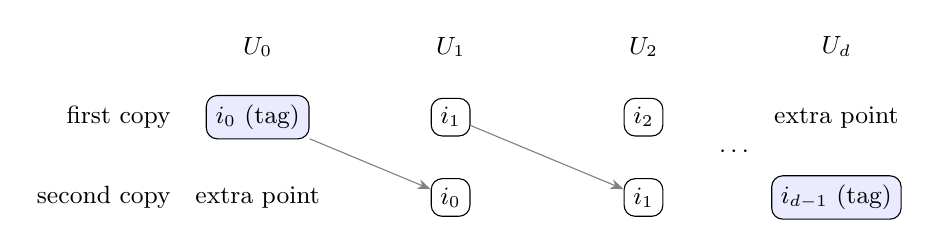
\begin{tikzpicture}[x=2.45cm,y=.85cm,>=Stealth,
  every node/.style={font=\small}]
 \foreach \x/\txt in {0/{U_0},1/{U_1},2/{U_2},3/{U_d}} {
   \node at (\x,1.05) {$\txt$};
 }
 \node[anchor=east] at (-.4,0) {first copy};
 \node[anchor=east] at (-.4,-1.2) {second copy};
 \node[draw,rounded corners,fill=blue!8] (a0) at (0,0) {$i_0$ (tag)};
 \node[draw,rounded corners] (a1) at (1,0) {$i_1$};
 \node[draw,rounded corners] (a2) at (2,0) {$i_2$};
 \node at (3,0) {extra point};
 \node at (0,-1.2) {extra point};
 \node[draw,rounded corners] (b1) at (1,-1.2) {$i_0$};
 \node[draw,rounded corners] (b2) at (2,-1.2) {$i_1$};
 \node[draw,rounded corners,fill=blue!8] (b3) at (3,-1.2) {$i_{d-1}$ (tag)};
 \draw[->,gray] (a0) -- (b1);
 \draw[->,gray] (a1) -- (b2);
 \node at (2.48,-.52) {$\cdots$};
\end{tikzpicture}
\caption{The two midpoint assignments. Each departure label moves one cell
along the path in the second copy; the drawing suppresses the intermediate
cells before $U_d$. Removing the highlighted tags leaves the same bath
midpoints. Each vertical column is one proposal factor, with a common
midpoint and one path in each copy when both are required.}
\label{cmp:shift-figure}
\end{figure}

\subsection{Cancellation of conditional normalizers}

The midpoint construction has two path copies in each internal vertex
factor. To estimate its likelihood, designate one copy as primary and regard
the other as auxiliary. At an internal vertex $z_k$, $1\le k<d$, the
primary path has label $i_k$ in the first-copy view, whereas the auxiliary
path has label
$i_{k-1}$. Thus deleting a factor is not the same operation as deleting all
instances of one particle label. The following lemma keeps this distinction
explicit and isolates the normalizers that cancel when two routes are far
apart. Its coordinates and factors are abstract; we identify them with the
midpoint construction immediately after the proof.

The next lemma concerns finitely many coordinates in standard Borel spaces,
each with a probability reference $P_i$. All auxiliary spaces below are
standard Borel as well. A \emph{check} will mean an indicator imposing a constraint
on one or two coordinates. The joint reference law $\lambda$ is the product
$\bigotimes_iP_i$ conditioned on a finite collection of checks. An additional
independent coordinate is allowed; it simply has no checks.

A change indexed by a set $S$ leaves the marginal outside $S$ unchanged.
Inside $S$, it starts from independent factors $\Pi_{S,i}$, $i\in S$.
Each factor includes a \emph{primary coordinate} in the space of $P_i$ and
possibly auxiliary coordinates. Its primary marginal is $g_{S,i}P_i$, with
\begin{equation}\label{cmp:factor-density}
 0\le g_{S,i}\le G,
 \qquad \int g_{S,i}\dd P_i=1.
\end{equation}
The factors are fixed before the outside coordinates are sampled. The product
is conditioned on specified checks, including every reference check involving
the primary coordinates in $S$. Checks involving only fixed outside
coordinates are already satisfied almost surely under the unchanged outside
marginal; otherwise the conditional proposal would not be defined there.
Omit these redundant checks. Every remaining proposal check therefore
involves a coordinate carried by a changed factor. Auxiliary coordinates
are then forgotten.
The resulting primary likelihood relative to $\lambda$ is denoted by $L_S$.

For each primary and auxiliary coordinate, fix a measurable allowed set
on which all its relevant reference and proposal marginals are
concentrated. These sets, like the proposal factors, are fixed before
sampling outside coordinates. A configuration is \emph{individually
permitted} when each coordinate lies in its allowed set; this imposes no
pairwise checks. The compatibility hypothesis below is uniform on these
sets, including configurations that fail some pairwise checks.

We make explicit the deletion convention for this construction. When some
factors are removed, remove their coordinates and all checks incident to them.
Do not replace a removed auxiliary coordinate by an original reference
coordinate. Coordinates fixed outside the sets under discussion remain as
obstacles in all the checks in which they occur. Coordinates here are path
instances in a specified copy. If an auxiliary with label $j$ belongs to a
retained factor, it remains integrated in that factor even when a different
factor carrying the primary label $j$ is deleted. It is never replaced by
the original path with label $j$.

\begin{lemma}[Cancellation away from an overlap]\label{cmp:cancellation}
Consider two changes $S,T$ of the preceding kind, with $G\ge1$, and put
$U=S\cup T$. Suppose that the following conditions hold.
\begin{enumerate}[label=\textup{(\roman*)}]
 \item There is $\chi\in[0,1)$ such that inserting any coordinate of $U$
 from its reference $P_i$, or any factor of either proposal from its
 $\Pi_{S,i}$ or $\Pi_{T,i}$, satisfies all checks incident to that insertion
 with probability at least $1-\chi$. This bound is uniform in every fixed
 choice of the other individually permitted coordinates. It remains valid
 when any checks or coordinates have been deleted.
 \item There are decompositions $S=C_S\sqcup F_S$ and
 $T=C_T\sqcup F_T$, with $F_S\cap T=F_T\cap S=\varnothing$.
 No coordinate carried by an $F_S$ factor has a check with any coordinate
 carried by a $T$ factor, or with the original primary coordinates indexed
 by $T$; the corresponding assertion holds with $S,T$ interchanged.
 The reference coordinates in $F_S,F_T$ also have no mutual checks.
\end{enumerate}
Then
\begin{equation}\label{cmp:cancellation-bound}
 \int L_SL_T\dd\lambda
 \le G^{|S\cap T|}(1-\chi)^{-2(|C_S|+|C_T|)}.
\end{equation}
It is enough that the assumptions hold for almost every fixed admissible
configuration outside $U$.
\end{lemma}

\begin{proof}
Put $a_\chi=1-\chi$ and $c=|C_S|+|C_T|$. Fix the primary coordinates
outside $U$. All normalizers below are conditional on these fixed values;
we first work on a configuration for which this conditional law is defined.

For any selected set, its reference normalizer is the integral of its
reference-check indicator against its product references. In particular,
write $Z_U$ for this integral over $U$. When the coordinates outside $S$
are fixed, write $Z_S$ for the corresponding integral over $S$. Thus $Z_S$
can depend on coordinates in $T\setminus S$. Write $Y_S$ for the integral
of the proposal-check indicator $J_S$ against $\bigotimes_{i\in S}\Pi_{S,i}$,
with the same outside values fixed.

Disintegrate each factor in the form
\[
 \Pi_{S,i}(\dd x_i\,\dd\zeta_i)
   =P_i(\dd x_i)K_{S,i}(x_i,\dd\zeta_i),
 \qquad K_{S,i}(x_i,\text{all})=g_{S,i}(x_i).
\]
Here $\zeta_i$ denotes all its auxiliary coordinates. Define
\[
 H_S(x_S;x_{S^c})
  =\int J_S\prod_{i\in S}K_{S,i}(x_i,\dd\zeta_i).
\]
On the reference-admissible configurations, the exact likelihood is
\begin{equation}\label{cmp:exact-likelihood}
 L_S=\frac{Z_S}{Y_S}H_S.
\end{equation}
Indeed, the conditional reference density is its check indicator divided by
$Z_S$, whereas the new primary density is $H_S/Y_S$, both relative to
$\bigotimes_{i\in S}P_i$. The outside marginal is identical. The inclusion
of primary reference checks ensures that the new density is zero on
reference-forbidden configurations.

Now retain only the factors indexed by $F_S$, together with coordinates fixed
outside $U$, using the stated deletion convention. Denote their reference
normalizer, proposal normalizer and primary proposal density by
$Z_{F_S},Y_{F_S},H_{F_S}$. Define the three corresponding $F_T$ quantities
using the factors from the $T$ change. These quantities depend only on the
outside of $U$ and, for $H_{F_S},H_{F_T}$, on their own primary coordinates.
They do not depend on the omitted near coordinates.

Successive insertion using assumption~\textup{(i)}, and noninteraction in
assumption~\textup{(ii)}, give
\begin{align}
 Z_U&\ge a_\chi^c Z_{F_S}Z_{F_T},
       \label{cmp:union-normalizer}\\
 Z_S&\le Z_{F_S},\qquad
 Y_S\ge a_\chi^{|C_S|}Y_{F_S},
       \label{cmp:single-normalizers}\\
 Z_T&\le Z_{F_T},\qquad
 Y_T\ge a_\chi^{|C_T|}Y_{F_T}.
       \label{cmp:other-normalizers}
\end{align}
For the first inequality, the reference integral over the two far sets
factorizes; add every remaining distinct coordinate with its uniform
compatibility bound. There are at most $c$ such coordinates. For the upper
bound on $Z_S$, delete the checks involving $C_S$ and integrate those reference
coordinates freely. Coordinates in $T\setminus S$ have no checks with the
far set. For its proposal lower bound, start with the reduced $F_S$ integral
and add the $C_S$ factors. The fixed original coordinates in
$T\setminus S$ still do not meet the far factors. Each addition retains at
least the factor $a_\chi$. Applying these two arguments to the $T$ change proves the
last line. These statements are pointwise in the opposing coordinates;
they do not assert that $Z_S$ or $Y_S$ is constant in them.

The insertion bounds also prove positivity of the divisors. In particular,
integrating coordinates one at a time gives a positive product lower bound
for every reduced normalizer. The full reference conditional is defined on
the outside configurations under consideration.

Deleting proposal checks involving a near factor gives
\[
 H_S\le H_{F_S}\prod_{i\in C_S}g_{S,i},
 \qquad
 H_T\le H_{F_T}\prod_{i\in C_T}g_{T,i}.
\]
After dropping the reference admissibility indicator in an upper bound,
the two far primary integrals equal $Y_{F_S}$ and $Y_{F_T}$. The remaining
coordinates carry only the displayed marginal densities. A coordinate
occurring once integrates to one. A coordinate occurring in both lists
costs at most $G$, by \eqref{cmp:factor-density}. Therefore
\begin{equation}\label{cmp:kernel-product}
 \int H_SH_T\ind_{\mathrm{admissible}}
              \prod_{i\in U}P_i(\dd x_i)
 \le Y_{F_S}Y_{F_T}G^{|S\cap T|}.
\end{equation}
The conditional reference law on $U$ has normalizer $Z_U$. Combine
\eqref{cmp:exact-likelihood}--\eqref{cmp:kernel-product}. The two pointwise
ratio bounds contribute
$a_\chi^{-c}Z_{F_S}Z_{F_T}/(Y_{F_S}Y_{F_T})$; division by $Z_U$
contributes at most $a_\chi^{-c}/(Z_{F_S}Z_{F_T})$. All four far
normalizers cancel, leaving $G^{|S\cap T|}a_\chi^{-2c}$.
Finally integrate the outside coordinates. This proves
\eqref{cmp:cancellation-bound}.
\end{proof}

\subsection{The likelihood cost is confined to encounters}

Fix the data, the route and the selected labels. Regard either copy as the
primary one. The reference for that copy is
$\lambda_{\cI}\otimes P_*$, where $P_*$ is the uniform law of the extra
point in its endpoint cell. Let
\[
 S=\{i_0,\ldots,i_{d-1}\}\cup\{*\}.
\]
The objects in Lemma~\ref{cmp:cancellation} now have the following meaning:
\begin{center}
\begin{tabular}{@{}p{.24\linewidth}p{.70\linewidth}@{}}
\toprule
Primary coordinate & The chosen copy's path, or its endpoint extra point.\\
Auxiliary coordinate & The other copy's path or extra point through the same midpoint.\\
Checks & Collision exclusions within each copy.\\
\bottomrule
\end{tabular}
\end{center}
Index a vertex factor by its primary label, using $*$ for the extra point;
its center is its midpoint cell $z_k$. The two paths in one factor may have
different labels, and each copy contributes at most one path. The allowed
set for each path consists of the regular, confined, frozen-avoiding paths
with its own recorded endpoints. Each extra point lies in its target cell.
These are individual restrictions; the remaining collision checks still
couple different factors.

By Proposition~\ref{group:comparison}, the primary marginal of each path
factor has density at most $G$ relative to $P_i$, and integrates to one.
For the extra point the density is $\ind_{A_k}/|A_k|$ relative to $P_*$,
which is at most $1/0.98$. Enlarge the fixed $G$ to be at least two, covering
this factor as well. These marginal densities and their auxiliary kernels
depend on the exposed data and the route and label choices; they do not
depend on the unselected unexposed paths.

The union bound proving Equation~\eqref{cmp:compatibility} verifies
hypothesis~\textup{(i)} for each proposal factor. The same argument with
$P_i$ in place of $\Pi_i^{A_k}$ verifies it for insertion of a selected
reference path, by Proposition~\ref{group:comparison}. The reference extra
point has no checks. These estimates are uniform over all individually
permitted opponent paths, whether or not their labels are accessible, and
deleting checks can only improve them. Thus the bound remains available
for every reduced normalizer in Lemma~\ref{cmp:cancellation}.

Take two independent route and label choices at the same data and endpoint
pair, and denote their selected index sets by $S,T$. For the chosen primary
side, declare a factor of $S$ near if its center is at lattice supremum
distance at most $R$ from some center of $T$, and declare every other factor
far. Define $C_S,F_S,C_T,F_T$ accordingly. A shared real label has centers
at distance at most two in the two assignments, so it is near; the shared
extra index has the same endpoint center. Consequently the far index sets
are disjoint from the opposing lists.

All paths carried by a factor lie within distance eleven of its center.
The original path of an opposing real label also lies within distance eleven
of that opposing factor's center. Since $R=30$, far factors cannot interact
with any coordinate carried by the opposite list or with those original
paths. This includes the auxiliary-copy paths. Far sets therefore meet the
separation assumptions of Lemma~\ref{cmp:cancellation}.

For clarity, a reduced far proposal retains exactly the paths carried by
its far vertex factors and the fixed paths outside $S\cup T$. It deletes
the omitted near factors in both copies. It does not put their original
trajectories back as unselected obstacles. With this convention all the
normalizers in \eqref{cmp:union-normalizer}--\eqref{cmp:kernel-product}
are the ones arising from the present construction.

Write $L_S,L_T$ for the two primary likelihoods. If
\[
 J_R=\#\{(j,k):d_\infty(z_j,z'_k)\le R\},
\]
then $|C_S|+|C_T|\le2J_R$. Lemma~\ref{cmp:cancellation} gives, at the
fixed data,
\begin{equation}\label{cmp:two-choice-bound}
 \int L_SL_T\dd(\lambda_{\cI}\otimes P_*)
 \le G^{|S\cap T|}(1-\chi_D)^{-4J_R}.
\end{equation}
In particular, no factor is paid for a long portion of one route that stays
away from the other.

\subsection{Averaging labels and forgetting the paths}

Condition on the data and the two lattice paths before choosing their labels.
Each common departure cell has at least $M/2$ accessible labels. The two
uniform choices at that cell match with probability at most $2/M$, and the
match events are independent between distinct common cells. Real labels
anchored at different cells cannot agree. The shared extra point contributes
one factor $G$, so
\begin{equation}\label{cmp:label-average}
 \E_{\mathrm{labels}}G^{|S\cap T|}
 \le G\exp\left(\frac{2(G-1)}M J_R\right).
\end{equation}
Choose the fixed integer $M$ sufficiently large for the good-site supply
and for
\begin{equation}\label{cmp:M-choice}
 \frac{2(G-1)}M\le\frac\kappa2.
\end{equation}
Then increase $D_0$ so that, for every $D\ge D_0$ in the allowed $\alpha$
window, all earlier estimates hold and
\begin{equation}\label{cmp:D-choice}
 -4\log(1-\chi_D)\le\frac\kappa2,
 \qquad
 \frac{G_D}{D}\ge\frac\ell{8M}.
\end{equation}
The first requirement is possible by \eqref{cmp:compatibility}; the second
follows once $\ell D/(4M)\ge2$. These choices do not change $G$, $\kappa$,
or $C_{\mathrm{path}}$.

The following use of an averaged likelihood and a two-route second moment
also occurs in the point-reassignment argument of
Peres and Sly~\cite[Proposition~2.1]{PeresSly2014}. Here
Lemma~\ref{cmp:cancellation} supplies the additional conditional-normalizer
estimate required by the hard-core path law.

Let $\overline L$ be the likelihood averaged over the conditional route and
label choices, with value zero off $\mathcal E_{vw}$. Tonelli's theorem
expresses its square integral using two independent such choices. Combining
\eqref{cmp:two-choice-bound}--\eqref{cmp:D-choice} and the annealed encounter
bound in Proposition~\ref{lat:paths} gives
\begin{equation}\label{cmp:latent-second-moment}
 \E_{\cB}\int\overline L^{2}
           \dd(\lambda_{\cI}\otimes P_*)
 \le G\E\bigl[\ind_{\mathcal E_{vw}}e^{\kappa J_R}\bigr]
 \le C_2,
 \qquad C_2:=G C_{\mathrm{path}}.
\end{equation}
Here the two route randomizations share the same data; the expectation over
the data is taken only once. The event is not conditioned to have probability
one. Its indicator is part of both likelihoods, and its square is itself.
The calculation applies separately with either copy primary, with the same
constant $C_2$.

We next check carefully that tagging and observing the bath do not increase
this bound. At fixed data, split $\overline L=\sum_{i\in\cI}f_i$, where
$f_i$ contains exactly the choices designating $i$ as the primary tag.
The functions are nonnegative. In the first copy $f_i$ is supported where
$\omega_i(t)\in B_v$; in the second it is supported where
$\omega_i(t)\in B_w$. Since
\[
 \sum_i f_i^2\le\left(\sum_i f_i\right)^2,
\]
the measure that retains the tag index has squared likelihood integral at
most $C_2$ relative to the \emph{sum} of the tag-restricted reference
measures on the disjoint copies indexed by $i$. Now apply the observation kernel that orders the bath and retains
$\cB,x,y,Y$, and forget the tag and all the paths. If a finite measure has
density $f$ relative to a reference $P$, the density after applying a common
kernel is the conditional average of $f$ in the corresponding joint
reference measure. Conditional Cauchy--Schwarz bounds its squared integral
by $\int f^2\dd P$. This remains valid for finite reference measures,
by normalization when their mass is nonzero.

For either primary copy, the resulting measure is the common observed
$\widehat\nu$ already constructed. Its corresponding reference is precisely
$\widehat P_g$ or $\widehat Q_g$. We have proved
\begin{equation}\label{cmp:observed-second-moments}
 \int\left(\frac{\dd\widehat\nu}{\dd\widehat P_g}\right)^2
                \dd\widehat P_g\le C_2,
 \qquad
 \int\left(\frac{\dd\widehat\nu}{\dd\widehat Q_g}\right)^2
                \dd\widehat Q_g\le C_2.
\end{equation}
Together with \eqref{cmp:common-mass}, Lemma~\ref{cmp:holder} now gives
\begin{equation}\label{cmp:one-group-gain}
 \Aff(\widehat P_g,\widehat Q_g)\ge\frac1{4C_2}.
\end{equation}
This lower bound is uniform in the group index and in every admissible
ordered pair of cells.

\begin{proposition}[Uniform modulus occupation]\label{cmp:modulus}
After the fixed choices above, there are constants $D_0<\infty$ and
\begin{equation}\label{cmp:c-star}
 c_*:=\frac{\upsilon_0\ell}{32M G C_{\mathrm{path}}}>0,
 \qquad \upsilon_0=\frac1{2000}
\end{equation}
such that, whenever $D\ge D_0$, $\alpha=Dr\in[\alpha_0/2,2\alpha_0]$,
and $K$ is sufficiently large, every normalized nonnegative bosonic ground
function satisfies $B(\Phi)\ge c_*$. The constant $c_*$ is unchanged if
the lower threshold on $D$ is subsequently increased. The volume thresholds
can be taken locally uniform for $D$ in compact subintervals of
$[D_0,\infty)$.
\end{proposition}
\begin{proof}
For large $K$, at least $\upsilon_0V^2$ ordered cell pairs meet the displacement
condition of Proposition~\ref{lat:paths}. For each such pair,
Lemma~\ref{cmp:tag-normalization}, \eqref{cmp:D-choice} and
\eqref{cmp:one-group-gain} give
\[
 \Aff(P_{vw},Q_{vw})
 \ge\frac{G_D}{4D C_2}
 \ge\frac\ell{32M C_2}.
\]
Sum these nonnegative contributions in \eqref{cmp:cell-affinity} to obtain
$B(\Phi)\ge\upsilon_0\ell/(32M C_2)$, which is \eqref{cmp:c-star}.
All ingredients are uniform in the ground vector. The threshold and
local-uniformity assertions follow from the preceding path and group
estimates and Proposition~\ref{lat:paths}. No parameter entering $c_*$ is
chosen after $D_0$.
\end{proof}

The modulus occupation has now been bounded below by a fixed number. To
treat the original complex ground vector, it remains to show that a small
part of each one-coordinate slice contains every possible phase obstruction.
That estimate may require a larger lower bound on $D$; Proposition~\ref{cmp:modulus}
permits that increase without changing the gain.

\section{A common component in each one-particle slice}
\label{geom:section}

We now construct the retained sets required by
Lemma~\ref{setup:phase-transfer}. With the bath fixed, we cover its
forbidden balls by microscopic cubes and fill the bounded pockets enclosed
by each bad cluster. The retained points will lie in one component of the
open allowed slice. To bound the removed volume, we separate clusters
whose coordinate spans are at most one from larger clusters. The former
cost at most $Cr^2N$ in total filled volume. Each larger cluster forces order
$1/r$ distinct nearby bath particles with close partners, so the joint
spatial estimates control its occurrence. This argument requires no
connectivity of the full configuration space.

We retain the scaled torus $\Lambda_K$, its volume $V=K^3$, and the centered
unit cells $B_v$, where $v\in(\Z/K\Z)^3$. Write
\[
 Y=(x_2,\ldots,x_N),\qquad
 m(Y)=\int_{\Lambda_K}\Phi(x,Y)^2\dd x,\qquad
 \nu(\dd Y)=m(Y)\dd Y.
\]
Thus $\nu$ is the bath marginal of $\mu(\dd X)=\Phi(X)^2\dd X$.
Call a bath admissible if $d(x_i,x_j)>r$ for $2\le i<j\le N$.
Other baths have $m(Y)=0$. For an admissible bath, its open
one-coordinate slice is
\begin{equation}\label{geom:allowed-slice}
 S_Y=\Lambda_K\setminus\bigcup_{j=2}^N\overline B(x_j,r).
\end{equation}
We first work deterministically with admissible baths. The probability
estimate at the end uses the joint close-neighbor bound from
Equation~\eqref{sp:close-tail}.

\subsection{Microcubes and filled components}

Put
\[
 q_r=\lceil1/r\rceil,\qquad h=q_r^{-1},\qquad J=Kq_r.
\]
For $r\le1$, we have $r/2\le h\le r$. Subdivide every unit cell into
$q_r^3$ microcubes. In the periodic lift, their closed cubes are
\[
 Q_z=h\bigl(z+[0,1]^3\bigr)-(1/2,1/2,1/2),\qquad z\in\Z^3.
\]
Their index period is $J$ in every coordinate. A microcube is \emph{bad}
if its closure intersects a closed ball in~\eqref{geom:allowed-slice};
otherwise it is \emph{good}. Marking is periodic. Distinct index sites are
$*$-adjacent when their maximum coordinate distance is one. For a finite
bad $*$-component $C$, let $H_\infty(C)$ be the unique infinite
nearest-neighbor component of $\Z^3\setminus C$, and put
\[
 \operatorname{Fill}(C)=\Z^3\setminus H_\infty(C).
\]
Thus the fill adds all finite nearest-neighbor holes to $C$.
Define $\cA(Y)\subset\Lambda_K$ as the projection of all closed cubes with
indices in the fills of the bad components. If the lifted bad set has an
infinite component, define $\cA(Y)=\Lambda_K$. Use this convention also
for inadmissible baths. The retained region is
\[
 G(Y)=\Lambda_K\setminus\cA(Y).
\]

The fills remove bounded pockets behind the obstacles. This is the same
discrete filling operation used in Lemma~\ref{lat:boundary}; here its scale
is comparable to the exclusion distance. Phase transfer requires the
points of $G(Y)$ to lie in one component of $S_Y$; a connecting path
may use any good microcubes. Figure~\ref{geom:figure} distinguishes bad
cubes, their fill, and such a route.

\begin{figure}[t]
\centering
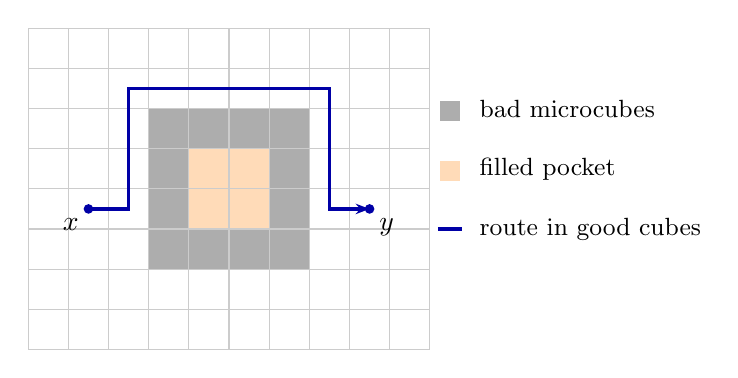
\begin{tikzpicture}[scale=.51]
 \foreach \x/\y in {3/2,4/2,5/2,6/2,3/3,6/3,3/4,6/4,3/5,4/5,5/5,6/5}
   \fill[black!32] (\x,\y) rectangle +(1,1);
 \fill[orange!28] (4,3) rectangle (6,5);
 \draw[black!20,step=1] (0,0) grid (10,8);
 \draw[very thick,blue!65!black,-{Stealth[length=5pt]}]
   (1.5,3.5)--(2.5,3.5)--(2.5,6.5)--(7.5,6.5)--(7.5,3.5)--(8.5,3.5);
 \fill[blue!65!black] (1.5,3.5) circle (.12) (8.5,3.5) circle (.12);
 \node[below left] at (1.5,3.5) {$x$};
 \node[below right] at (8.5,3.5) {$y$};
 \node[anchor=west] at (11,6) {\small bad microcubes};
 \fill[black!32] (10.25,5.7) rectangle +(0.5,0.5);
 \node[anchor=west] at (11,4.5) {\small filled pocket};
 \fill[orange!28] (10.25,4.2) rectangle +(0.5,0.5);
 \node[anchor=west] at (11,3) {\small route in good cubes};
 \draw[very thick,blue!65!black] (10.2,3)--(10.8,3);
\end{tikzpicture}
\caption{A planar schematic of the filling operation. The argument uses
three-dimensional microcubes. Each closed good cube avoids every closed
forbidden ball, so a finite route through good cubes has positive clearance.
The picture concerns a single-coordinate slice with the bath fixed.}
\label{geom:figure}
\end{figure}

\begin{lemma}[Connectivity with strict clearance]\label{geom:connectivity}
For every bath $Y$, any two points of $G(Y)$ can be joined by a continuous
path in $S_Y$ whose distance from the forbidden set is strictly positive.
\end{lemma}

\begin{proof}
There is nothing to prove when $G(Y)$ is empty. Otherwise the bath is
admissible and all lifted bad components are finite. Choose lifted microcube
sites containing the two points. Each lies outside the fill of every lifted bad component, and hence
in its infinite nearest-neighbor complement component.

Start with any finite nearest-neighbor path between these sites. If it
visits a bad component $C$, let $u$ precede the first visit and let $w$
follow the last visit. The path prefix before $u$ avoids $C$ and connects
$u$ to an endpoint outside its fill. The reversed suffix does the same for
$w$. Thus both vertices belong to the exterior $*$-boundary of $C$ visible
from infinity by nearest-neighbor paths. Lemma~\ref{lat:boundary} joins
them by a nearest-neighbor path in this boundary. All its vertices are
good: a bad $*$-neighbor of $C$ would already be in $C$.

This replacement removes bad vertices and introduces none. Repetition
therefore terminates, since the original path had finitely many bad
vertices. First and last visits are taken for one fixed lifted component;
different periodic copies are treated separately. Projecting the resulting
good-cube path gives a route on the torus.

Join successive cube centers through their common faces, and join the
original points to their cube centers. A point on a grid face can be
assigned any adjacent cube: membership outside $\cA(Y)$ ensures that each
such cube is good and outside every fill. Every closed good cube is
disjoint from every closed forbidden ball. The finite union of cubes used
by the route is compact, so its distance from the union of the closed
forbidden balls is positive. All the line segments stay in these cubes. This proves both
open-slice connectivity and strict clearance.
\end{proof}

\subsection{Small fills and distinct close-particle witnesses}

Call a finite microcomponent $C$ \emph{small} if
$h\diam_\infty C\le1$. All other components, including infinite ones,
are called \emph{large}. For a small fill, each occupied column has
cross-sectional area $h^2$ and length at most order one; charging each
occupied column to a bad cube gives the deterministic volume bound below. Large
components will instead force the close-neighbor events already estimated
under $\mu$.

\begin{lemma}[Volume of small fills]\label{geom:small-fills}
For $K>10$ and $r\le1$, the projected union of small fills has volume at
most $C r^2 N$, with an absolute constant $C$.
\end{lemma}

\begin{proof}
The fill of a finite component lies in its coordinate bounding box by
Lemma~\ref{lat:boundary}. Moreover, every column parallel to the first
coordinate axis that meets the fill also meets the component. Otherwise
that entire column would avoid the component and connect each of its
vertices to infinity, precluding a finite hole there.

For a small component $C$, there are at most $|C|$ such columns. Each
contributes length at most $1+2h$ in physical units and cross-sectional
area $h^2$. Hence its filled cubes have volume at most
\begin{equation}\label{geom:column-volume}
 (1+2h)h^2|C|\le3h^2|C|.
\end{equation}
A closed radius-$r$ ball meets at most $C_0=343$ microcubes, since
$r/h\le2$ and in each coordinate at most seven closed grid intervals
can meet its projection.

Choose one representative of each small component modulo the torus
period. Its projection is injective because each physical coordinate span
is at most one and $K>10$. The projected components are disjoint, and their
total number of bad microcubes is at most $C_0(N-1)$. Summing
Equation~\eqref{geom:column-volume}, and allowing overlaps of their
fills in this upper bound, gives $3C_0h^2(N-1)\le C r^2N$.
\end{proof}

\begin{lemma}[Distinct witnesses in a large component]
\label{geom:large-witnesses}
There are absolute constants $r_1,c_{\rm g}>0$ such that the following
holds for $r\le r_1$ and $K>10$. If a unit cell $B_v$ contains a
microcube from a large bad component, then at least $c_{\rm g}/r$
distinct bath particles lie within distance $5$ of $v$, and each has a
distinct bath particle within distance $6r$.
One may take $c_{\rm g}=1/(8C_0)$ with $C_0=343$.
\end{lemma}

\begin{proof}
Fix a lifted microcube index $z$ in that component and in a lift of $B_v$.
There is a component vertex at scaled maximum distance greater than
$1/2$ from $z$. For a finite component this follows from its diameter
being greater than one; for an infinite component it follows from local
finiteness. Follow a simple $*$-path from $z$, stopping when its scaled
maximum distance first reaches $1/4$. It contains at least $1/(4h)$
distinct vertices and remains within scaled distance $1/4+h$ of $z$.

Choose one bath ball witnessing badness at each path vertex. A fixed ball
witnesses at most $C_0$ of these vertices. All the chosen centers are in
a fixed small neighborhood of $v$, contained in its radius-$5$ ball for
sufficiently small $r$. This neighborhood and the cubes under consideration
have diameter less than $K$, so no two periodic copies of the same label
occur. The witness sequence therefore contains at least
$1/(4C_0h)\ge1/(4C_0r)$ distinct labels. Shrink $r_1$ so this number is
at least two, and retain the stated smaller constant $c_{\rm g}$.

Repeated labels do not destroy the close-partner conclusion. Form a graph
whose vertices are the distinct witness labels, joining different labels
whenever they occur consecutively in the sequence. This graph is connected
and has at least two vertices, so none is isolated. Two adjacent closed
microcubes meet. The centers of balls intersecting those cubes are therefore
at distance at most
\[
 2r+2\sqrt3\,h\le6r.
\]
Every distinct label thus has a different close partner, including labels
that recur in separated portions of the witness sequence.
\end{proof}

We now fix the geometric restriction on the close-count threshold:
\begin{equation}\label{geom:theta-choice}
 0<\theta<\frac{c_{\rm g}}{2\alpha_0}.
\end{equation}
This restriction is imposed before the choice of $b$ in the spatial
estimates. Since $r=\alpha/D$ and $\alpha\le2\alpha_0$, increasing
the lower threshold on $D$ ensures
\begin{equation}\label{geom:scale-separation}
 6r<s_0=bD^{-1/3},\qquad r\le r_1.
\end{equation}
For a full configuration $X=(x,Y)$, recall the close-count set from
Equation~\eqref{sp:close-bad-set}:
\begin{equation}\label{geom:coarse-bad-set}
 \mathcal Q(X)
 =\left\{v:\#\left\{i:d(x_i,v)\le5,
                    \min_{j\ne i}d(x_i,x_j)\le s_0\right\}
                   \ge\theta D\right\}.
\end{equation}
By Equation~\eqref{sp:close-tail}, for every deterministic set $S$ of
distinct coarse sites,
\begin{equation}\label{geom:coarse-joint-bound}
 \mu\{S\subset\mathcal Q(X)\}\le p_D^{|S|},
 \qquad p_D\longrightarrow0.
\end{equation}
Lemma~\ref{geom:large-witnesses} and
Equations~\eqref{geom:theta-choice}--\eqref{geom:scale-separation}
show that every parent cell of a large microcomponent belongs to
$\mathcal Q(X)$. Indeed $c_{\rm g}/r>\theta D$, and adding
the distinguished point $x$ to the bath can only decrease the relevant
nearest-neighbor distances. This implication holds for every $x$; it does
not identify $\nu$ with an $(N-1)$-particle ground-state law.

\subsection{Periodic animals and the omitted volume}

\begin{proposition}[Small omitted volume]\label{geom:omitted-volume}
Fix the constants as above and take $D$ sufficiently large. There are
absolute constants $C,C_{\rm an}$ such that, for $K\ge100$ and
$C_{\rm an}p_D\le1/2$,
\begin{equation}\label{geom:volume-bound}
 \delta_{\rm geom}:=\int\frac{|\cA(Y)|}{V}\,\nu(\dd Y)
 \le C r^2D+C p_D
       +K^3(C_{\rm an}p_D)^{\lfloor K/10\rfloor}.
\end{equation}
The retained points belong to one component of the open slice
$S_Y$ whenever the retained set is nonempty. The estimate is uniform
over the normalized ground vector and $\alpha\in[\alpha_0/2,2\alpha_0]$.
\end{proposition}

\begin{proof}
We estimate the bath-dependent volume by integrating under the full
configuration law:
\begin{equation}\label{geom:bath-volume-identity}
 \delta_{\rm geom}
 =\int_{\Lambda_K^N}\frac{|\cA(Y)|}{V}\,\mu(\dd x\,\dd Y).
\end{equation}
This is the marginal identity $\int\Phi(x,Y)^2\dd x=m(Y)$.
The coarse bad events used next may therefore depend on $x$ as well
as on the bath.

Set $m_K=\lfloor K/10\rfloor$ and let $\mathcal E_K$ be the event
that the coarse bad set in~\eqref{geom:coarse-bad-set} has a
$*$-component of size at least $m_K$. In a graph of degree $26$, the
number of connected vertex sets of size $m$ containing a prescribed root
is at most $C_{\rm an}^m$. To see this, choose for each set a deterministic
spanning tree and its depth-first traversal: the resulting walk has
$2(m-1)$ steps, and its visited set recovers the original set. There are
at most $26^{2(m-1)}$ such walks. A connected set of size at least $m_K$
contains a connected subset of size exactly $m_K$, by taking the first
$m_K$ vertices in a tree exploration. Equation~\eqref{geom:coarse-joint-bound}
and a union bound over roots give
\begin{equation}\label{geom:large-animal-error}
 \mu(\mathcal E_K)
 \le K^3(C_{\rm an}p_D)^{m_K}.
\end{equation}

On $\mathcal E_K^c$, every coarse bad component has fewer than $K/10$
vertices. We make its periodic lifting explicit. Lift a spanning tree of
a component with $m$ vertices. Each additional edge and its tree path
form a loop of length at most $2m-1<K$. Such a loop has zero winding:
every step changes each coordinate by at most one, whereas nonzero winding
requires displacement of magnitude at least $K$ in one coordinate.
Every additional edge therefore closes in the chosen finite tree lift.
This proves that the full lifted component is finite, projects bijectively,
and has coordinate span at most $m-1$. It is the nearest-range case of
Lemma~\ref{lat:small-lifts}.

The parent-cell map sends adjacent microcubes to equal or $*$-adjacent
unit cells. Every large microcomponent is therefore contained in the unit
cubes of one lifted coarse bad component. In particular it is finite on
$\mathcal E_K^c$: each of those finitely many unit cubes contains only
$q_r^3$ microcubes. Its fill lies in its own coordinate bounding box and
thus in the coordinate box of those unit cubes.

Consequently, if a prescribed unit cell is affected by a large fill,
there is a coarse bad animal of some size $m\ge1$ with a root within
maximum distance $C m$ of that cell. There are at most $C m^3$ possible
roots, even after projecting to the torus. The rooted-animal count and
Equation~\eqref{geom:coarse-joint-bound} give
\begin{equation}\label{geom:filled-animal-sum}
 \mu\{\mathcal E_K^c\text{ and the cell meets a large fill}\}
 \le\sum_{m\ge1} C m^3(C_{\rm an}p_D)^m\le C'p_D.
\end{equation}
The last inequality follows by summing the convergent power series on
$C_{\rm an}p_D\le1/2$. No independence of coarse sites is used.

Sum Equation~\eqref{geom:filled-animal-sum} over unit cells and divide
by $V$. On $\mathcal E_K$, bound the discarded fraction by one.
Lemma~\ref{geom:small-fills} bounds the small-fill contribution by
$Cr^2N/V=Cr^2D$. Combining these bounds with
Equation~\eqref{geom:large-animal-error} proves
Equation~\eqref{geom:volume-bound}, by
Equation~\eqref{geom:bath-volume-identity}.
Lemma~\ref{geom:connectivity} gives the connectivity assertion.

All sets used here are measurable. Bad-cube membership is a finite family
of distance tests in one period. A finite periodic component has a finite
lift precisely when its spanning-tree lift closes along every additional
edge. In that case its fill is determined by connectivity in a finite
bounding box, with the exterior attached. These finite procedures determine
the projected discarded cubes and their volume from the bath positions.
\end{proof}

The right side of Equation~\eqref{geom:volume-bound} has the needed order
of limits. Since $r^2D=\alpha^2/D$, its first two terms can be made
arbitrarily small by increasing the lower threshold on $D$. At each such
fixed density, the last term tends to zero as $K$ grows. Its displayed
bound also gives uniform convergence for all $D$ above a threshold at
which $C_{\rm an}p_D\le1/2$. The estimate is therefore ready for the
phase-transfer lemma and the final parameter choice.

\section{Choice of constants and the thermodynamic limit}\label{main:conclusion}

We now combine the uniform modulus bound with the phase estimate. The
order of the choices is essential: the modulus fraction is fixed before
we make the discarded volume small enough to preserve it.

\subsection{A bound in the scaled variables}

\begin{proposition}\label{main:scaled}
There are absolute constants $\alpha_0,D_*,c_*>0$ such that, for
$D=N/K^3\ge D_*$ and $r=\alpha/D$ with
$\alpha\in[\alpha_0/2,2\alpha_0]$, every normalized complex bosonic
ground vector satisfies
\[
 B(\Psi)\ge c_*/2
\]
for all sufficiently large integer $K$. The volume threshold can be
chosen uniformly when $D$ ranges over a fixed compact subinterval of
$[D_*,\infty)$, and is independent of the chosen ground vector.
\end{proposition}

\begin{proof}
We first list the choices that yield Proposition~\ref{cmp:modulus}.
Fix the local cutoff profiles and the exponent $\gamma=1/12$ in the
path regularity conditions. Choose $\alpha_0$ large enough for the
insertion and spatial estimates, and then choose the small lower-count
constant $\ell$. Choose the close-count threshold $\theta$ so that
\[
 3\theta<\ell/2,\qquad \theta<c_{\rm g}/(2\alpha_0).
\]
The first inequality leaves the required eligible labels; the second
is the witness condition in Equation~\eqref{geom:theta-choice}.
Next fix the separation constant $b$ in $s_0=bD^{-1/3}$.

At the fixed encounter radius $R=30$, Proposition~\ref{lat:paths}
supplies a bad-site tolerance $p$, an exponential-moment parameter
$\kappa>0$, and a bound $C_{\rm path}$. Fix the visitor threshold
$H_1$ and the regularity threshold in the certificate estimates, and
then the small time $t>0$ in the bridge estimates. All these constants
are fixed before $D$ is increased. The local comparison bound
$G\ge2$ of Proposition~\ref{group:comparison} is now fixed as well.
Choose the integer group size $M$ large enough for the grouping
failure estimate and for
\[
 \frac{2(G-1)}M\le\frac\kappa2.
\]
Finally choose $D_0$ large enough for all the preceding estimates, for
$\ell D\ge8M$, and for
\[
 -4\log(1-\chi_D)\le\frac\kappa2,
 \qquad \chi_D=C_{\rm col}M\eta_D.
\]
Here $\eta_D\to0$ is the deterministic-opponent collision bound from
Proposition~\ref{group:comparison}. We may replace each vanishing error by
its nonincreasing upper envelope, so these requirements hold for all
$D\ge D_0$.

Proposition~\ref{cmp:modulus} then gives
\begin{equation}\label{main:cstar}
 B(\Phi)\ge c_*:=\frac{\upsilon_0\ell}{32M G C_{\rm path}}>0,
 \qquad \upsilon_0=\frac1{2000}.
\end{equation}
None of $\upsilon_0,\ell,M,G,C_{\rm path}$ changes when the lower threshold on
$D$ is subsequently increased.

By Proposition~\ref{geom:omitted-volume}, the retained points lie in a
common component of each allowed slice, and their discarded-volume
expectation satisfies
\begin{equation}\label{main:geometry-error}
 \delta_{\rm geom}
 \le C\frac{\alpha^2}{D}+C p_D
       +C K^3(C_{\rm an}p_D)^{\lfloor K/10\rfloor},
 \qquad p_D\longrightarrow0.
\end{equation}
The constants in this estimate use only choices already fixed.
Increase $D_0$ to $D_*$ so that, for every $D\ge D_*$ and every
$\alpha$ in its fixed window,
\[
 C\frac{\alpha^2}{D}+Cp_D\le\frac{c_*^2}{256},
 \qquad C_{\rm an}p_D\le\frac12.
\]
For sufficiently large $K$ the last term in
Equation~\eqref{main:geometry-error} is at most $c_*^2/256$.
In particular $\delta_{\rm geom}\le c_*^2/64$, and
Lemma~\ref{setup:phase-transfer} gives $B(\Psi)\ge c_*/2$.

Proposition~\ref{cmp:modulus} supplies volume thresholds locally
uniform in $D$, independently of the ground vector and of $\alpha$
in its fixed window. The geometric restrictions above hold for all
$D\ge D_*$, and the remaining volume error is uniformly at most
$C K^3 2^{-\lfloor K/10\rfloor}$. Combining these two facts proves
the asserted local uniformity in $D$ for the complex ground vector.
\end{proof}

\subsection{Return to fixed exclusion distance and density}

\begin{proof}[Proof of Theorem~\ref{main:theorem}]
Let $\alpha_0,D_*,c_*$ be the constants of
Proposition~\ref{main:scaled}, and set
\[
 \varepsilon_0=\frac{\alpha_0^3}{4D_*^2},\qquad c_0=c_*/2.
\]
Decrease $\varepsilon_0$ if needed to meet the fixed dilute-regime
prerequisites. Fix $a,\rho>0$ with $\rho a^3<\varepsilon_0$, and
let $N_k,L_k,\Psi_k$ be any sequence in the theorem.
We choose the integer side to keep the product of scaled density and
exclusion distance close to $\alpha_0$.
Equation~\eqref{setup:gas-parameter} will then turn the small physical
gas parameter into a large scaled density.
For all sufficiently large $k$ define
\[
 q_k=\sqrt{\frac{aN_k}{\alpha_0 L_k}},\qquad
 K_k=\lfloor q_k\rfloor,\qquad
 r_k=\frac{aK_k}{L_k},\qquad D_k=\frac{N_k}{K_k^3}.
\]
Since $q_k/L_k\to\sqrt{a\rho/\alpha_0}>0$, we have
$K_k\to\infty$ and $K_k/q_k\to1$. Consequently
\begin{align*}
 \alpha_k:=D_kr_k
   &=\frac{aN_k}{L_kK_k^2}
     =\alpha_0\left(\frac{q_k}{K_k}\right)^2
       \longrightarrow\alpha_0,\\
 D_k&\longrightarrow
       D_\infty:=\frac{\alpha_0^{3/2}}{\sqrt{\rho a^3}}
       >2D_*.
\end{align*}
Thus $\alpha_k$ lies in the required window and $D_k$ lies in a
compact subinterval of $(D_*,\infty)$ for all sufficiently large
$k$. The local uniformity in Proposition~\ref{main:scaled} applies to
this varying sequence of scaled densities.

Use the unitary change of length from Section~\ref{setup:section},
with $s_k=L_k/K_k$. It carries $\Psi_k$ to a normalized bosonic
ground vector on $\Lambda_{K_k}$ with exclusion distance $r_k$, and
preserves $B$. Proposition~\ref{main:scaled} therefore gives
$B(\Psi_k)\ge c_0$ for all sufficiently large $k$.
The argument is uniform over the choice of ground vector, so it proves
Equation~\eqref{main:limit} for every such sequence.
\end{proof}

\begin{proof}[Proof of Corollary~\ref{main:mixed}]
The bosonic ground eigenspace is finite dimensional by compactness of
the form embedding. Every density operator supported on it is a convex
combination of rank-one projections onto normalized ground vectors.
For all sufficiently large members of the sequence, the proof of
Theorem~\ref{main:theorem} gives the same lower bound $c_0$ for each
of those vectors. Constant-orbital occupation is linear in the density
operator. The lower bound therefore holds for their convex combination,
including $\Pi_k/\Tr\Pi_k$. A nonnegative ground vector is already
covered by the theorem.
\end{proof}

\bibliographystyle{plainnat}
\bibliography{references}
\end{document}
